\documentclass[a4paper,titlepage,twoside,fleqn,12pt]{book}

% format of the thesis
  %\usepackage{classicthesis} % --- check for compatibility with noweb
\usepackage{titlesec}
\usepackage[a4paper,margin=1in]{geometry}
\usepackage[T1]{fontenc}
\usepackage[british]{babel}

\usepackage{fancyhdr}
\setlength{\headheight}{28.7pt}
\pagestyle{fancy}
\fancyhf{}
\fancyhead[LE,RO]{Book}
\fancyhead[RE,LO]{Cos}
\fancyfoot[CE,CO]{}
\fancyfoot[LE,RO]{\thepage}

\renewcommand{\headrulewidth}{1.4pt}
\renewcommand{\footrulewidth}{0.0pt}

\widowpenalty=300
\clubpenalty=300

% font of the text: charter, times, fourier*, palatino
\usepackage{fourier}

% hyphenation
\usepackage{hyphenat}
\hyphenation{di-men-sio-nal}
\hyphenation{e-lec-tro-sta-tic sol-va-to-chro-mic sol-va-to-chro-mism}
\usepackage[shortcuts]{extdash}
\frenchspacing

% chapter format
\usepackage[Sonny]{fncychap}
\ChNameVar{\Huge\bf}
\ChNumVar{\fontsize{70}{60}\selectfont}
\ChTitleVar{\huge\bf}
\ChRuleWidth{1.5pt}
\ChNameAsIs
% rubberband spaces between paragraphs
%\setlength{\parskip}{3ex plus 2ex minus 2ex}

% section numbers and table of contents 
\setcounter{secnumdepth}{3} 
\setcounter{tocdepth}{2}

% appnendices
\usepackage[toc,page]{appendix}

% bibliography
%\usepackage{natbib}
\usepackage[natbib=true,style=chem-acs,sorting=none]{biblatex}
\addbibresource{bibliography.bib}

% literate programming
\usepackage{noweb}

% graphics
\usepackage{graphicx}

% tables
\usepackage{dcolumn}

% mathematics
\usepackage{amsmath}
\usepackage{amsfonts}
\usepackage{amssymb}
\usepackage{mathrsfs}

% symbols
\usepackage{gensymb}

% footnotes
\usepackage[symbol]{footmisc}

% caption fonts
\usepackage[font=scriptsize,labelfont=bf]{caption}

% annoying page breaks leaving blank pages
\def\nwendcode{\endtrivlist\endgroup}
\let\nwdocspar=\relax

% navigation pane in PDF file
\usepackage{hyperref}
\hypersetup{
    pdftitle={PhD Thesis},
    pdfauthor={Bartosz Błasiak},
    pdfsubject={Your subject here},
    pdfkeywords={vibrational solvatochromism, interaction energy, ab initio, quantum chemistry},
    bookmarksnumbered=true,     
    bookmarksopen=true,         
    bookmarksopenlevel=1,       
    colorlinks=false,            
    pdfstartview=Fit,           
    pdfpagemode=UseOutlines,
    pdfpagelayout=TwoPageRight
}
\usepackage{hypcap}

%---------------------------------------------------
% SHORTCUTS
\newcolumntype{,}{D{.}{,}{2}}
\newcommand{\citee}[1]{\ensuremath{\scriptsize^{\citenum{#1}}}}
\newcommand{\HRule}{\rule{\linewidth}{0.5mm}}
% Quantum notation
\newcommand{\bra}[1]{\ensuremath{\bigl\langle {#1} \bigl\lvert}}
\newcommand{\ket}[1]{\ensuremath{\bigr\rvert {#1} \bigr\rangle}}
\newcommand{\braket}[2]{\ensuremath{\bigl\langle {#1} \bigl\lvert {#2} \bigr\rangle}}
\newcommand{\tbraket}[3]{\ensuremath{\bigl\langle {#1} \bigl\lvert {#2} \bigl\lvert {#3} \bigr\rangle}}
% Math
\newcommand{\pd}{\ensuremath{\partial}}
\newcommand{\DR}{\ensuremath{{\rm d} {\bf r}}}
\newcommand{\BM}[1]{\ensuremath{\mbox{\boldmath${#1}$}}}
% Chemistry (formulas)
\newcommand{\ch}[2]{\ensuremath{\mathrm{#1}_{#2}}}
% Math 
\newcommand{\VEC}[1]{\ensuremath{\mathrm{\mathbf{#1}}}}
% vector nabla
\newcommand{\Nabla}{\ensuremath{ \BM{\nabla}}}
% derivative
\newcommand{\FDer}[3]{\ensuremath{
\bigg(
\frac{\partial #1}{\partial #2}
\bigg)_{#3}}}
% diagonal second derivative
\newcommand{\SDer}[3]{\ensuremath{
\biggl(
\frac{\partial^2 #1}{\partial #2^2}
\biggr)_{#3}}}
% off-diagonal second derivative
\newcommand{\SSDer}[4]{\ensuremath{
\biggl(
\frac{\partial^2 #1}{\partial #2 \partial #3}
\biggr)_{#4}}}
%---------------------------------------------------

% subtitle
\usepackage{titling}
\newcommand{\subtitle}[1]{%
  \posttitle{%
    \par\end{center}
    \begin{center}\large#1\end{center}
    \vskip0.5em}%
}

% title
\title{Molecular Solvatochromism}
\subtitle{Vibrational Frequency Shift Theory}
\author{Bartosz B{\l}asiak}

%---------------------------------------------------
\begin{document}
%---------------------------------------------------
\graphicspath{{figures/}}
%---------------------------------------------------
\maketitle
%---------------------------------------------------
\tableofcontents
%---------------------------------------------------

\chapter*{Preface}

This Thesis is addressed to everyone who wants to understand the physical
origins of the vibrational solvatochromism phenomenon. Or in other, more specific words, 
the aim of this work is to quantitatively link the changes in the infra\hyp{}red (IR)
spectral signal with the gas-phase molecular properties such as electron energy and charge
density distribution and, of course, their vibrational characteristics. 

This Thesis is not only a theoretical dissertation. It is also a working program 
in which the first-principles theory of vibrational solvatochromic frequency shift is 
implemented. Therefore, I provide a Tutorial with examples how to use {\sc Solvshift} 
since the Reader might want to extend the functionality of the program in the future.
The current version of the program is limited only to the estimation of the vibrational frequency 
shifts in the cases when we can neglect the solvation-induced intramolecular mode mixing.

% ==== CHAPTER 1

\begin{refsection}
\chapter{Introduction}

Modeling the reality of single, isolated molecules have been 
an intensive and extremely fascinating field of science over the
last century. The birth of quantum mechanics by Bohr and Dirac enabled the unprecedensed
before nanoscale theoretical tool that can deal with objects as small
as atoms and molecules. Quantum chemistry pioneered by Fock, Roothaan, Hartree, Hall
and Pople achieved solving the Schr{\"o}dinger
equation with sometimes breathtaking precisions when compared to experiment.
From that moment, the molecular properties such as charge distributions, ionization energies,
electronic affinities, vibrational modes and electromagnetic susceptibilities
have become within reach of researchers (and even laics!).\footnote{due to the
sharply growing, often open-source, colourful palette of quantum chemistry software
written in a diversity of computer languages -- from Fortran77 and C++ to Python and Ruby.} 

However, the reality is not just about the single molecules. It is more about their aggregates,
how they interact and form complex, extended systems. Taking into account such enormous
amounts of electrons and putting it all together into the Schr{\"o}dinger equation 
is unfortunately far beyond the capabilities of nowadays' computers. So, how can we solve this 
(seemingly) unsolvable problem? 

In 1958 Buckingham stated\citep{Buckingham.ProcRSocLondonA.1958} that
%
\begin{quote}
\emph{
[\ldots] the energy levels and transition moments of isolated molecules are often 
of interest, so it has been worthwile to attempt to relate the spectra of compressed
gasses, solutions, pure liquids and solids to the properties of independent molecules.
}
\end{quote}
%
Therefore, we can use spectroscopy to study the intermolecular interactions
if we know the fundamental principles that govern the interaction-induced molecular property
change. In fact, there is a lot of such properties that could be traced when changing
the molecular partners around the spectator molecule: from its
structure, charge distribution and transition frequencies to electric\slash{}magnetic 
susceptibilities with non\hyp{}linear optical properties in particular.
%Or, in other words, 
%\begin{quote}
%Can we say anything about the molecule $A$ surrounded by other molecules $B$
%basing only on their intrinsic properties (i.e. when they are \emph{isolated})?
%\end{quote}

This Book is devoted to a special molecular characteristic 
that can be directly linked with the local molecular environment, mainly
the frequency of a particular vibrational transition, or, in short, 
vibrational frequency. 

This is extremely fascinating field of science, indeed. If we combine the
ultrafast time\hyp{}domain vibrational spectroscopy, that had emerged during the recent
two decades\citep{Book-Cho.TwoDimensionalOpticalSpectroscopy.2009}, 
with our thorough understanding of the \emph{vibrational solvatochromism},
we can interpret the experimental signal. What it gives us is the 
ability to extract the highly local site\hyp{}specific structural information
that can be traced in a sub-nanosecond resolution (generally in a range of
a few to tens of ps) which is kind of an ultrafast molecular motion picture.

To get such a deep insight into a molecular world '\emph{in vivo}' one needs
first to develop the detailed model which can link the vibrational frequency
with the change in the surroundings. The very first approximation is to use
electrostatic picture where the molecule in question responds to the applied
electric field (can be uniform or vary from place to place). The problem is that
the nature of a typical intermolecular interaction is far more complex than this. However, 
due to the complexity of the quantum theory, mainly electrostatic models
have been considered before. In this Thesis we go much further than the
electrostatic picture. The goal is to develop 
a more general description of the vibrational solvatochromism, that includes
not only Coulombic forces, but also other important phenomena. 
So, the final form of the 
question we will challenge to find answer for is as follows:
%
\begin{quote}
To what extent can we predict the vibrational properties of spectator molecule $A$ 
surrounded by (not in the least small amount of) other molecules $B$
basing only on their intrinsic electrostatic properties 
(i.e. when they are \emph{isolated})? \textbf{Do we need to include also other
contributions to the vibrational solvatochromism phenomenon that were not studied
in detail before?}
\end{quote}
%

This Thesis is two\hyp{}fold in its scope: i) it aims to maximally develop
the electrostatic model of vibrational solvatochromism and compare it
with the previous approximate analyses reported so far; ii) to
study effects that are not in correlation with electrostatic properties
of solute and solvent molecules at all. In Chapter~\ref{c:background} I will 
briefly review the state of understanding of the vibrational solvatochromism
before findings presented in this Thesis were published. In Chapter~\ref{c:background}
I will also (thoroughly) elaborate the underlying theory of the vibrational
solvatochromism that is the foundation of this Work. 

So, let's start!

\printbibliography[heading=subbibintoc,title={References}]
\end{refsection}

\begin{refsection}
\chapter{Vibrational Solvatochromism}

Molecules have various energetic properties that 
depend on their interactions with environment. In particular,
the transitions between vibrational quantum states
that involve absorption in the IR region of 
electromagnetic field also change. 
In this Chapter, we outline the phenomenon 
of the vibrational solvatochromism, i.e., the process of
the changes in the vibrational absorption spectrum upon the change 
of the molecular surroundings around an IR active spectator.

\section{Overview}
%
It was nearly eight decades ago when Bauer and Magat noticed 
that the vibrational frequencies
of solute tend to red-shift when
increasing the dielectric constant of the solvent.\citep{Bauer.Magat.JPhysRadium.1938} 
The latter is the macroscopic descriptor 
of how the environment (i.e., solvent molecules) is able to affect solute's 
electronic density distribution by means of the, so called, induction
effects. The larger value of $\varepsilon$ relative to its value in vacuum
($\varepsilon=1$) indicates stronger induction effects. 

Bauer and Magat found that in the limit of small deviations
from vacuum dielectric constant, the frequency change with respect to the
gas-phase state of $A$ is proportional to
%
\begin{equation} \label{e:kbm}
\Delta \omega(\varepsilon) \propto - \frac{\varepsilon-1}{2\varepsilon+1}
\end{equation}
%
where $\Delta\omega(\varepsilon) = \omega(\varepsilon) - \omega_0$ is the
angular frequency shift upon solvation with respect to the gas-phase frequency
$\omega_0$. The function $\frac{\varepsilon-1}{2\varepsilon+1}$ is also called
the Onsager factor. This relation is widely known as Kirkwood-Bauer-Magat (KBM) 
limiting law and is based on the Kirkwood-Onsager continuum model of 
solvation.\citep{Kirkwood.JCP.1934,Onsager.JACS.1936}

Let us take a closer look at KBM law and it's range of validity by analyzing the vibrational
solvatochromism based on certain example. As the Reader knows, the solute\hyp{}solvent intermolecular interactions 
depend strongly on the choice of the solvent.\citep{Stone.TheTheoryOfIntermolecularForces.1996,Gutmann.Resch.Linert.CoordChemRev.1982} 
Let us consider a solute molecule which has
only H\hyp{}bond\hyp{}acceptor sites (lone pairs on N or O atoms). These kinds of solute molecules
(nitriles, ketones, azides and so on) are remarkably useful in spectroscopy.

In the case of H\hyp{}bond\hyp{}accepting solutes, first type of solvents are the ones
which are non\hyp{}polar (dielectric constant is between 1.8-2.5) such as, for example,
hexane, CCl$_4$ or benzene\footnote{Aromatic solvents are somewhat special because 
of the delocalized $\pi$-electrons. Therefore, larger dispersion interactions are to be expected in general.
Increased dispersion effects can be possible also in the case of halogenated solvents}. 
These solvents are composed
of molecules having vanishing dipole moments. Therefore, the relevant forces that act on
solute molecule will be long\hyp{}range, rather non-specific polarization and dispersion
forces as well as short\hyp{}range van der Waals forces. 

The second class of the solvents can be divided into two subclasses. 
Weakly polar aprotic solvents ($\varepsilon$ between 4-20) 
like CHCl$_3$ (chloroform), fluorobenzene or tetrahydrofuran (THF), 
and strongly polar aprotic solvents like dimethylsulfoxide (DMSO) 
or MeCN (acetonitrile; $\varepsilon$ around 40).
The molecules of such solvents have certain, non-zero dipole moment 
which enables those molecules to form specific electrostatic interactions with 
solute molecules.

The third class of solvents are protic solvents which are always polar 
($\varepsilon$ between 40-80). The examples are water, ethanol or trifluoroacetic acid (TFA).
Those molecules can form specific H\hyp{}bonds with solute molecules. 

In Figure~\ref{f.MeCN.MeSCN.vs.solvents} we have gathered the vibrational 
frequencies of the nitrile (CN) stretch mode in methylocyanate (MeCN, known also as acetonitrile) and methylothiocyanate
(MeSCN) when dissolved in different solvents of varying polarity and proticity.\citep{Blasiak.Ritchie.Webb.Cho.XXX.2016}
The actual spectra are shown in the Appendix~\ref{a:exp-ftir} whereas here we focus only
on the frequency at peak maximum.
%
\begin{figure}[ht]
\centering
\setlength\fboxsep{0.4pt}
\setlength\fboxrule{0.5pt}
\fbox{
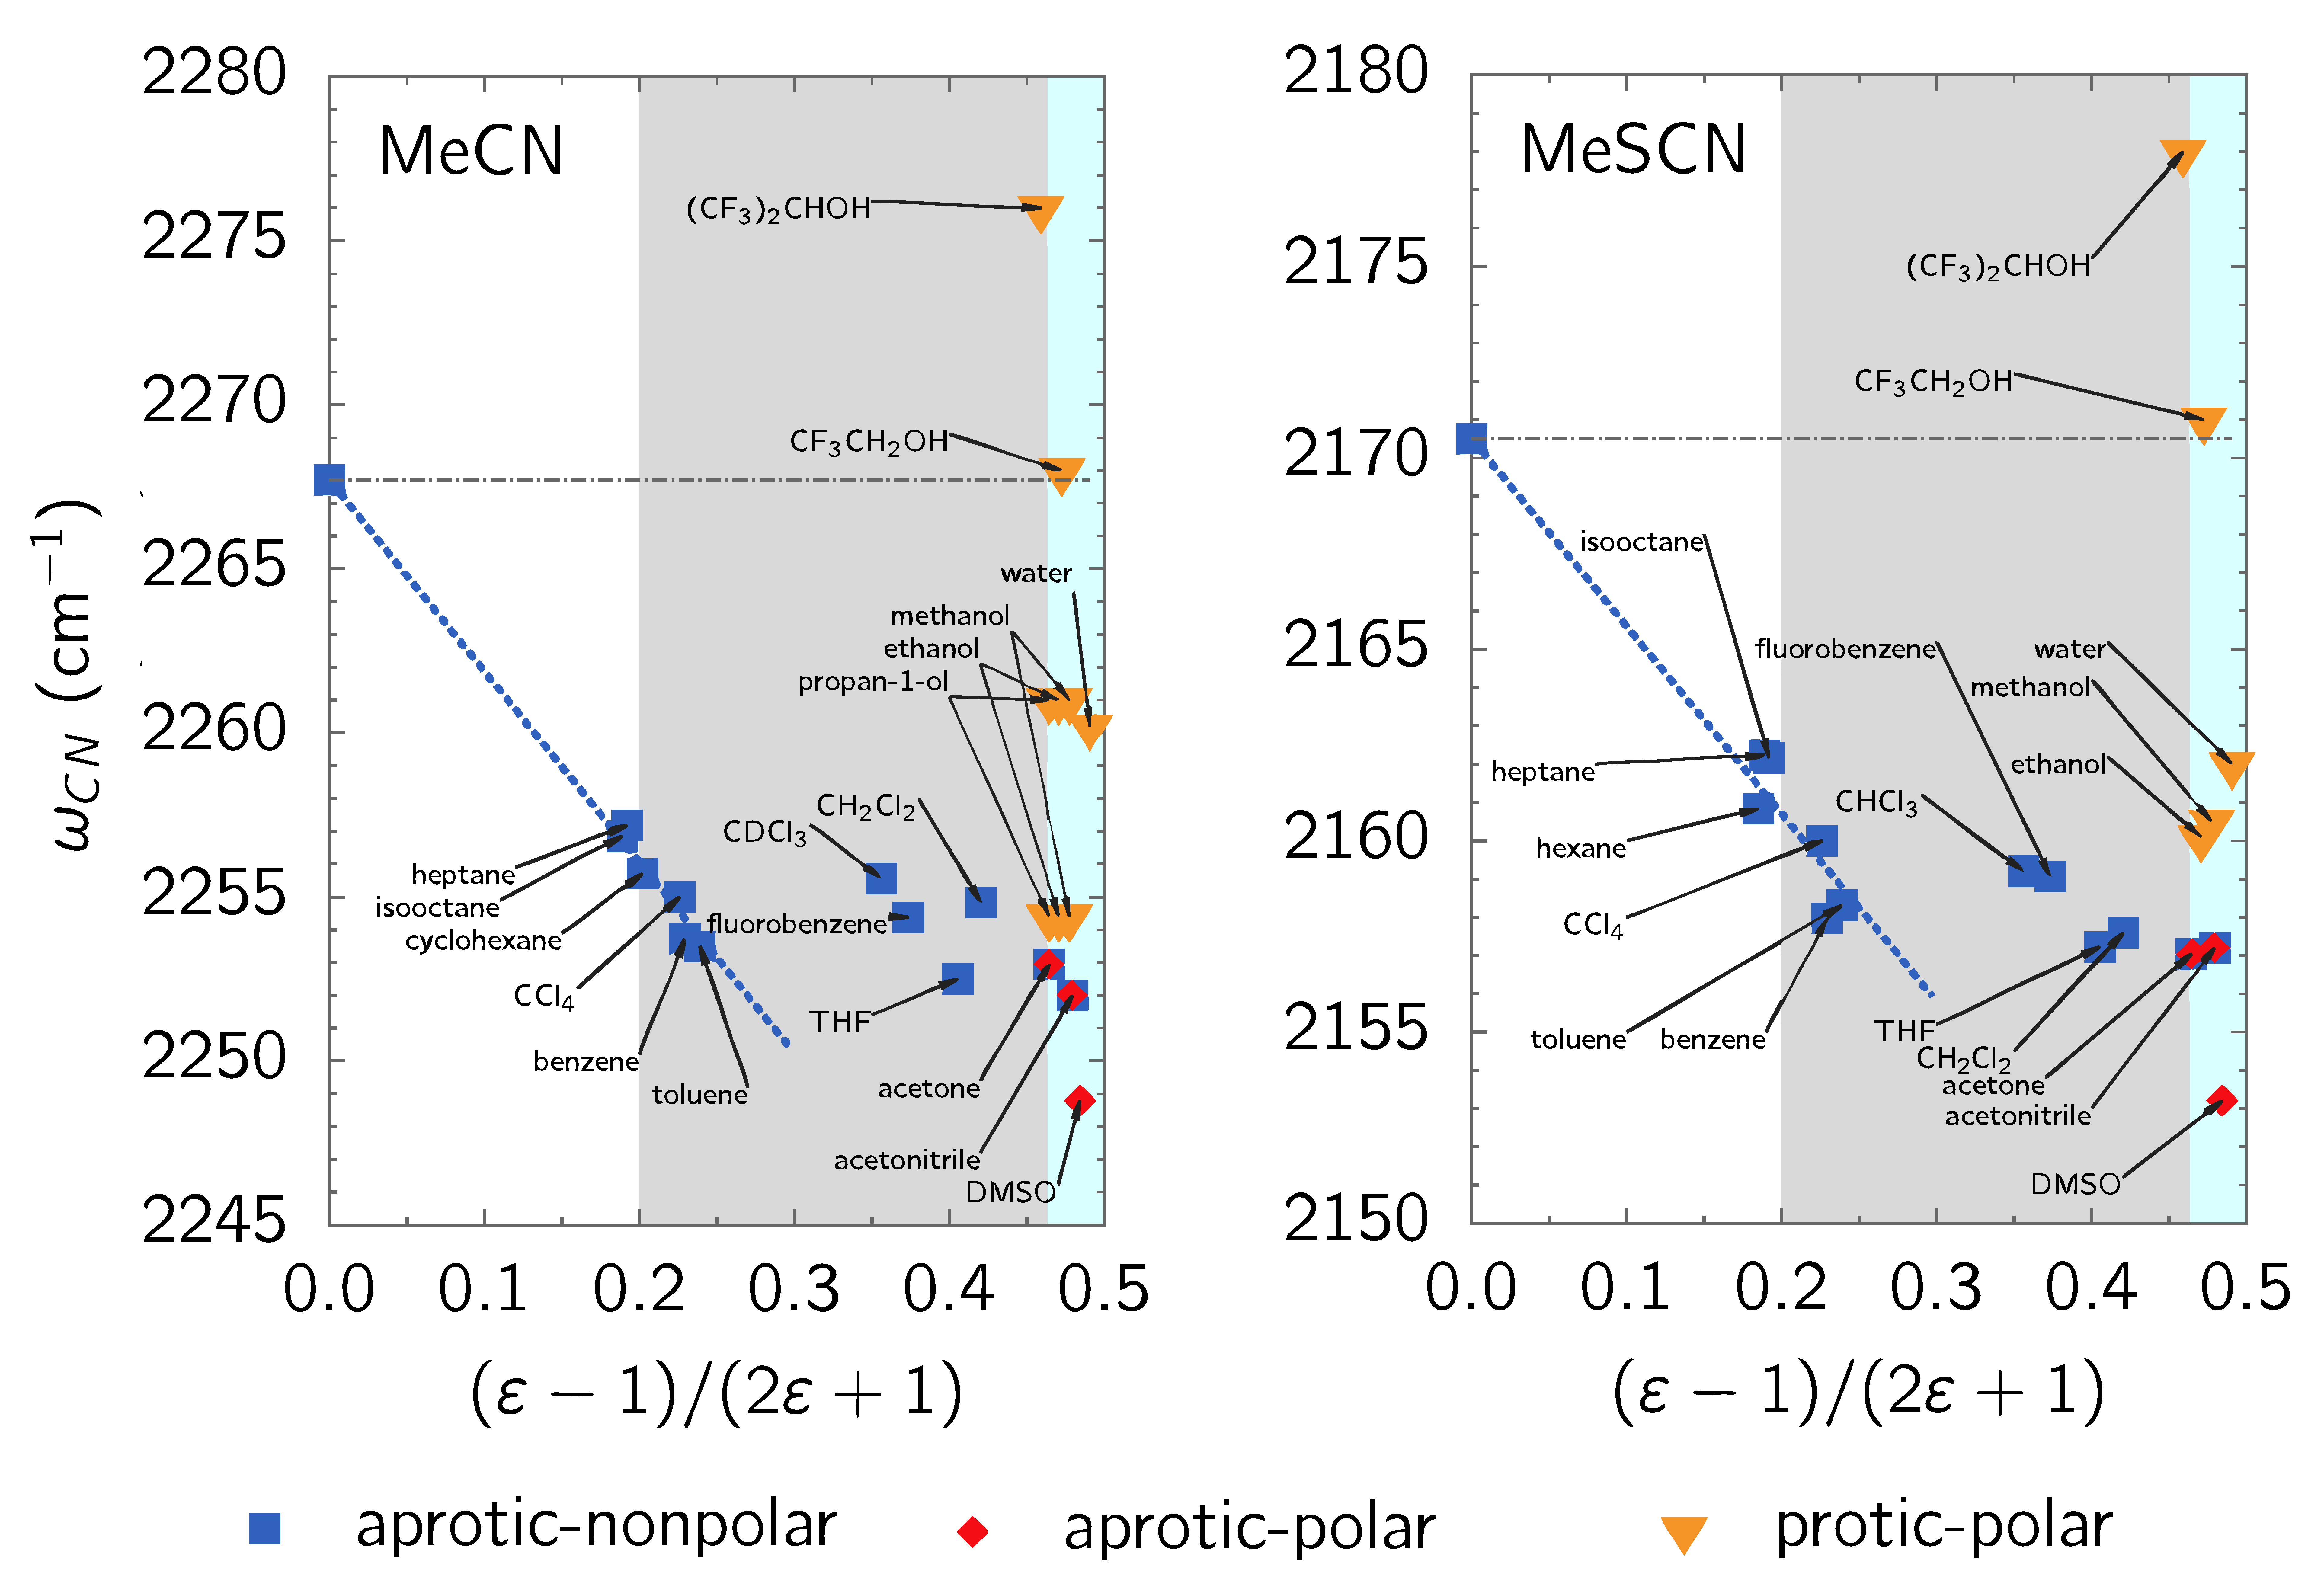
\includegraphics[width=0.9\linewidth]{Fig.1.eps}
}
\caption{Experimental frequencies of CN stretch mode of MeCN and MeSCN dissolved in
various solvents at room temperature. In this Figure, $\varepsilon$
stands for the solvent dielectric constant. Note that Onsager factor is zero in gas-phase. 
Frequencies that were not directly measured for this work were taken from the following 
References: MeCN in gas-phase (Refs.72-74), MeCN in CCl$_4$, THF, MeOH, H$_2$O, CF$_3$CH$_2$OH and 
(CF$_3$)$_2$CHOH (Ref.75), MeCN in CH$_3$(CH$_2$)$_2$OH (Ref.76), MeSCN in gas-phase (Ref.77), MeSCN in 
CCl$_4$, CHCl$_3$, CH$_2$Cl$_2$, MeCN, EtOH, MeOH, H$_2$O, CF$_3$CH$_2$OH and (CF$_3$)$_2$CHOH (Ref.78). In the 
cases of solvents with vanishingly small dipole moment (heptane, hexane, cyclohexane, 
isooctane, CCl$_4$), the linear relationship between CN frequency and Onsager factor indicates that 
the Kirkwood-Bauer-Magat law (blue line) works well.
\label{f.MeCN.MeSCN.vs.solvents}}
\end{figure}
%

As can be seen, for aprotic and non-polar solvents, the linear dependence of
nitrile frequency shift on the Onsager factor is evident, suggesting the validity of the KBM theory.
It is a great success of the apparently simplistic continuum model of solvation. 
However, as the solvent polarity increases, the reaction field 
theory for vibrational solvatochromism fails. Furthermore, as the H-bond donating ability of 
solvent molecule increases, the nitrile stretch frequency becomes strongly blue-shifted, as 
compared to those in DMSO for instance.\citep{Wilderen.Luuk.Kern-Michler.Muller-Werkmeister.Bredenbeck.PCCP.2014}
This just indicates that the continuum representation of the surroundings is not acceptable in general
because of the neglect of the, so called, specific solvation effects. 
They include the direct solute\hyp{}solvent intermolecular
contacts like collisions, directional electrostatic interactions and weak bonding (for instance, hydrogen- (H-) bonding).
Nevertheless, it is clear that vibrational frequency may be fairly sensitive 
to the solvent used, even when the change of the polarity is small.

The solvation of many simple molecules was studied experimentally in detail from the perspective of the 
vibrational properties of some particular localized vibration.\citep{Rowlen.Harris.AnalChem.1991,Mayne.Hudson.JPC.1991,
Janroz.Stangret.Lindgren.JACS.1993,Akiyama.Ohtani.SpectchimActA.1994,
Reimers.Hall.JACS.1999,Wilderen.Luuk.Kern-Michler.Muller-Werkmeister.Bredenbeck.PCCP.2014,Jansen.JPCB.2014} 
Owing to the vibrational solvatochromism
like in Fig.~\ref{f.MeCN.MeSCN.vs.solvents}, 
appropriately chosen vibrational chromophores, which can be either a small molecule or a small functional
group, can be used as a local reporters of their vicinity.\citep{Kim.Cho.ChemRev.2013} 
We shall refer to such interesting chromophores as to the infrared (IR) probes. 

\section{Infrared Probes}

Throughout the years, there have been quite a few IR probes found or synthesized, and
they are nowodays widely used to study various molecular environments, starting from bulk solutions
to proteins, nucleic acids and other polymers.\citep{Kim.Cho.ChemRev.2013,
Ma.Pazos.Zhang.Culik.Gai.AnnuRevPhysChem.2015,Waegele.Culik.Gai.JPCL.2011}
Among the functional gropus that have been demonstrated to be useful IR probes
are carbonyl (CO)\citep{Fried.Bagchi.Boxer.Science.2014,Thielges.Axup.Wong.Lee.Chung.Schultz.Fayer.JPCB.2011}, 
nitrile (CN)\citep{Zhang.Markiewicz.Doerksen.Smith.Gai.PCCP.2015,Johnson.Londergan.Charkoudian.JACS.2014,
Waegele.Culik.Gai.JPCL.2011,Stafford.Ensign.Webb.JPCB.2010,
Silverman.Pitzer.Ankomah.Boxer.Fenlon.JPCB.2007,Suydam.Snow.Pande.Boxer.Science.2006},
asymmetric azide (N$_3$)\citep{Thielges.Axup.Wong.Lee.Chung.Schultz.Fayer.JPCB.2011,
Ye.Zaitseva.Caltabiano.Schertler.Sakmar.Deupi.Vogel.Nature.2010,Waegele.Culik.Gai.JPCL.2011,
Taskent-Sezgin.Chung.Banerjee.Nagarajan.Dyer.Carrico.Raleigh.AngewChemInt.2010,Oh.Lee.Joo.Han.Cho.JPCB.2008} 
stretches, phosphate vibrations\citep{Levinson.Bolte.Miller.Corcelli.Boxer.JACS.2011}
and vibrations within nitro (NO$_2$) group\citep{Smith.Linderman.Luskin.Brewer.JPCB.2011}. 
Unique examples of using simultaneously two localized IR probes
were also reported.\citep{Thielges.Axup.Wong.Lee.Chung.Schultz.Fayer.JPCB.2011}
Those IR probes
generally fulfill the most important requirements for making it a useful tool: i) their transition
frequency is in the spectrally clean region, ii) their oscillatory strength is strong enough
to make them visible in the spectrum and analyze the signal, iii) the line shape 
of the resulting absorption peak is relatively easy to understand and has reasonably
narrow band width. 

Within the carbonyl IR probes, the first ever considered were the amide I modes
naturally occuring in proteins which are mostly the vibrations of the peptide group (CONH). Since
there is a lot of CONH groups in a protein, amide I modes can couple with each other
giving rise to the exciton bands in the IR spectra. This feature enabled to study 
the 3D structures of proteins with a combination of transition density
models\citep{Hayashi.Mukamel.JPCB.2007} because the coupling strongly depends 
on the relative orientation of transition dipoles. 
The problem with amide I mode (or amide I' when the proton becomes deuterated)
is that the linewidth is still relatively broad. In addition, it is impossible to
obtain the local structural information due to the couplings.

Different strategy of using IR probes is related to isolated CO, CN or N$_3$ groups.
CO groups can be genetically encoded
such as CO bound to heme metal center in myoglobin. 
CN and N$_3$ probes can be also site-selectively introduced into a macromolecular 
framework\citep{Jo.Culik.Korendovych.DeGrado.Gai.Biochem.2010,
Wang.Winblade.Johnson.Tirrell.Grabstein.ChemBioChem.2008,Fafarman.Webb.Chuang.Boxer.JACS.2006,
Kiick.Saxon.Tirrell.Bertozzi.PNAS.2002} 
which also provides
a local sond of the molecular environment. In particular, when such IR probe
is inserted into an active site of an enzyme, it becomes possible to study
how the enzyme acts within picosecond time scales.\citep{Fried.Bagchi.Boxer.Science.2014,Bagchi.Boxer.Fayer.JPCB.2012,
Ye.Zaitseva.Caltabiano.Schertler.Sakmar.Deupi.Vogel.Nature.2010} 
Another attractive way is to study protein structural fluctuation dynamics
or the protein-protein contacts when IR probe is localized at the protein 
surface\citep{Taskent-Sezgin.Chung.Banerjee.Nagarajan.Dyer.Carrico.Raleigh.AngewChemInt.2010,
Stafford.Ensign.Webb.JPCB.2010,Oh.Lee.Joo.Han.Cho.JPCB.2008}.  

\section{Understanding the Vibrational Solvatochromism}
%
However, the most fundamental issue that needs to be addressed 
before any IR probe is used, is what actually causes the vibrational solvatochromism.
Definitely, the electrostatic effects were considered to be the most important
(c.f. the KBM model) and much efforts were made to study the effects of the external
electric fields on the vibrational properties.\citep{Kim.Cho.ChemRev.2013} 
In particular, the effects of the
uniform external electric field was thoroughly examined.\citep{Hush.Reimers.JPC.1995,
Reimers.Zeng.Hush.JPC.1996,Andrews.Boxer.JCPA.2002,Cho.JCP.2009} 
In the vibrational Stark spectroscopy (VSE)\citep{Hush.Reimers.JPC.1995,Reimers.Zeng.Hush.JPC.1996}, 
which was pioneered experimentally by Boxer's laboratory\citep{Bublitz.Boxer.AnnuRevPhysChem.1997}, 
the change of the frequency, absorbance
and line shape is measured when the uniform external electric field is applied in certain fixed direction.
Under this circumstance, the frequency shift
was shown to be related to the electric field as follows\citep{Hush.Reimers.JPC.1995,Reimers.Zeng.Hush.JPC.1996}
%
\begin{equation} \label{e:vse-shift-full}
 \Delta \omega \approx - \Delta {\BM \mu} \cdot {\bf F} - \frac{1}{2} \Delta {\BM \alpha} : {\bf F} \otimes {\bf F}
\end{equation}
%
where $\Delta {\BM \mu}$ is, so called, the Stark tuning rate
and $\Delta {\BM \alpha}$ accounts for the quadratic effect with respect to 
the electric field, ${\bf F}$. 
Based on the VSE measurements, for the conventional
electric fields that exist inside biomolecules, the quadratic term
can be safely neglected. 
% CHECK THIS:
%For example, for the maximal electric field
%value reported so far (~160 MV/cm\citep{Fried.Bagchi.Boxer.Science.2014}) and the (assumed) upper bound for 
%$\Delta \alpha=1\times10^{-6}$ 
%cm$^{-1}\times \left({\rm cm}/{\rm MV}\right)^2$\citep{Andrews.Boxer.JCPA.2000,Andrews.Boxer.JCPA.2002}, 
%the frequency shifts is less than 0.03 cm$^{-1}$. For the sake 
%of comparison, the frequency shifts caused by linear term in Eq.~\eqref{e:vse-shift-full}
%can range from 3--100 cm$^{-1}$.
This fact gave rise to the dipole approximation (VSE-d)
widely used by VSE spectroscopists,
%
\begin{equation} \label{e:vse-shift-dipole}
 \Delta \omega \approx - \Delta {\BM \mu} \cdot {\bf F}
\end{equation}
%
Stark tuning rates have been reported for many IR probes.\citep{Suydam.Boxer.Biochem.2003,Levinson.Fried.Boxer.JPCB.2012}
They also were computed by using quantum chemistry calculations\citep{Dalosto.Vanderkooi.Sharp.JPCB.2004,
Andrews.Boxer.JCPA.2002,Andrews.Boxer.JCPA.2000}
and they are typically in a range of 0.4-1.0 cm$^{-1}$/(MV/cm). 
Since Eq.~\eqref{e:vse-shift-dipole} is proportional to solute's
dipole property, VSE-d have been correlated with Onsager's dipole
continuum model. For some subset of aprotic and non-polar
solvents descent linear correlation was found.\citep{Levinson.Fried.Boxer.JPCB.2012} 
Unfortunately,
when strongly protic solvents are used the significant deviations
from the linear correlations were observed.\citep{Fafarman.Sigala.Herschlag.Boxer.JACS.2010,Bagchi.Fried.Boxer.JACS.2012}

However, the serious drawback of VSE lies in the neglect of the field gradients that are 
likely to occur in the condensed phase. In fact, it was denomstrated theoretically
by Cho\citep{Cho.JCP.2009,Lee.Choi.Cho.JCP.2012} 
that when electric field varies in space, Eq.~\eqref{e:vse-shift-dipole}
has to be extended to account properly for field gradients,
%
\begin{equation} \label{e:vse-shift-multipoles}
 \Delta \omega 
\approx 
             - \Delta {\BM \mu}    \cdot               {\bf F} 
- \frac{1}{3}  \Delta {\BM \Theta} :      \nabla       {\bf F}
- \frac{1}{15} \Delta {\BM \Omega} \vdots \nabla\nabla {\bf F}
+ \ldots
\end{equation}
%
where the appropriate \emph{solvatochromic multipoles}
interact with the electric field ($\Delta {\BM \mu}$), 
field gradient ($\Delta {\BM \Theta}$), gradient of field gradient ($\Delta {\BM \Omega}$),
and so forth.
Another problem is related with the crude simplification of the 
molecular surroundings which is treated with continuum Onsager's model.
Despite all that, VSE is still being vividly
used by researchers to probe local electric fields in enzymes, DNA strands and 
lipid layers. 

There is yet another unclear issue which is associated with the electric field
used during the VSE experiment in order to determine Stark tuning rate.
It was shown that actually ${\bf F}$ is not perfetctly constant but varies
near the molecule. The reason for this is the local field effect that arises
from the response of the molecule that is exposed to the perturbing electric field.
This phenomenon is difficult to assess quantitatively. Therefore, 
the empirical scaling factor, so called local field correction factor, $f$, 
was introduced to modify Eq.~\eqref{e:vse-shift-dipole} as follows
%
\begin{equation} \label{e:vse-shift-dipole-corr}
 \Delta \omega \approx - f \Delta {\BM \mu} \cdot {\bf F}
\end{equation}
%
According to continuum Lorentz model, $f$ is given by\citep{Wortmann.Bishop.JCP.1998}
%
\begin{equation}
f(\omega) = \frac{n^2(\omega)+2}{3}
\end{equation}
%
where $n(\omega)$ is the frequency\hyp{}dependent refractive index.
In the limiting case $\omega=0$ $f$ can be also expressed according to Onsager
model as\citep{Wortmann.Bishop.JCP.1998}
%
\begin{equation}
f(0) = \frac{\varepsilon (n^2(0)+2)}{n^2(0)+2\varepsilon}
\end{equation}
%
It was deduced that $f$ can be in the range of 1.1-1.3\citep{Wortmann.Bishop.JCP.1998,
Bublitz.Boxer.AnnuRevPhysChem.1997}, although
it is unclear whether this is always the case.

It is possible to combine the vibrational spectroscopy of IR probes (mostly VSE) with nuclear magnetic 
resonance (NMR) technique, which was demonstrated by Boxer's 
group.\citep{Fafarman.Sigala.Herschlag.Boxer.JACS.2010,Bagchi.Fried.Boxer.JACS.2012} 
It enables one
to separate out the contributions from the H\hyp{}bonding and other effects. However, 
it is very difficult to use this technique since it refers to empirical observables only,
and hence, one cannot get any detailed insight into the intricacies of the molecular granularity
and types of residues around an IR probe.

A few empirical models of the vibrational solvatochromism has been developed throughout the years.
They employ a variety of fitting procedures with a few adjustable parameters. For example, 
models based on certain molecular descriptors such as polarity, Lewis\slash{}Br{\o}nsted acidity\slash{}basicity, 
H-bonding donating\slash{}accepting ability were shown to be quite useful in relating the vibrational
frequency and infrared intensity with the type of solvent used. Among many methods of this kind,
one can mention Kamlet\hyp{}Taft parameters\citep{Kamlet.Taft.JACS.1976,Taft.Kamlet.JACS.1976,Kamlet.Abboud.Taft.JACS.1977}, 
Fawcett's molecular descriptor method\citep{Reimers.Hall.JACS.1999,
Fawcett.Liu.Kessler.JPC.1993,Fawcett.Kloss.JCP.1996} or Ben Amotz' theory.\citep{Ben-Amotz.Lee.Cho.List.JCP.1992} 
The latter is actually derived from first principles, but it was mostly used by fitting
the resulting parameters to the experiment rather that explicitely obtaining them from calculations.
We will talk about the Ben Amotz' model in more detail later (Section XXX) because it is the first
truly first\hyp{}principles model that decomposes the frequency shifts into not only electrostatic, 
but also non-electrostatic repulsive contributions.

In KT parameter method, frequency shifts can be related to the following
relation\citep{Zhang.Markiewicz.Doerksen.Smith.Gai.PCCP.2015}:
%
\begin{equation} \label{e:kamlet-taft}
\Delta \omega = A\alpha + B\beta + C\pi^{*}
\end{equation}
%
In this approach, one has to
find the coefficients $A$, $B$ and $C$ that are fitted against
the solute's KT parameters $\alpha$\citep{Taft.Kamlet.JACS.1976}, 
$\beta$\citep{Kamlet.Taft.JACS.1976} and $\pi^{*}$\citep{Kamlet.Abboud.Taft.JACS.1977} 
describing the hydrogen bond accepting,
hydrogen bond donating, and dielectric interactions abilities, respectively.
KT parameters were originally determined from VIS spectra and related different
spectroscopic observables into one multivariate linear relationship as in Eq.~\eqref{e:kamlet-taft}.

Slightly more complicated parameterization was developed 
by Fawcett et al.\citep{Reimers.Hall.JACS.1999,Fawcett.Liu.Kessler.JPC.1993,Fawcett.Kloss.JCP.1996},
in which the solute's frequency shift\footnote{originally acetonitrile $\nu_2$ frequency
which is CN stretch mode} can be expressed by the mix of solute- and
solvent-related empirical descriptors
%
\begin{multline} \label{e:fawcett}
\Delta \omega = \Delta \omega_{gp} + 
\left( a_{Sol} - a_{St} \right) A_A +
\left( d_{Sol} - d_{St} \right) A_D \\ + 
\left( \frac{\varepsilon_{Sol}-1}{\varepsilon_{Sol}+2} - \frac{\varepsilon_{St}-1}{\varepsilon_{St}+2} \right) A_\varepsilon +
\frac{3}{4\pi}
\left( \frac{n^2_{Sol}-1}{n^2_{Sol}+1} - \frac{n^2_{St}-1}{n^2_{St}+1} \right) A_\alpha
\end{multline}
%
In the above formula, $\Delta \omega_{gp}$ denotes the frequency shift in pure liquid of solute
relative to the gas phase,
$a$ and $d$ are the Gutmann solvent acceptor and donor numbers\citep{Gutmann.Resch.Linert.CoordChemRev.1982}, 
respectively,
and the associated four constants $A_A$, $A_D$, $A_\varepsilon$ and $A_\alpha$ 
are to be fit to the experimentally determined frequency shifts in different solvents.
The lower indices $St$ and $Sol$ indicate solute and solvent parameters, respectively. 
Note that all fitting parameters in Eqs.~\eqref{e:kamlet-taft} and ~\eqref{e:fawcett} 
describe the solute-solvent interactions empirically.

In his seminal works, Ben-Amotz et al.\citep{Ben-Amotz.Lee.Cho.List.JCP.1992} 
used the first-principles theory of Buckingham
to derive the contributions to the vibrational frequency shift due to
repulsive, attractive and centrifugal distortion forces. Mainly,
%
\begin{equation} \label{e:ben-amotz}
 \Delta \omega = \Delta \omega_R + \Delta \omega_A + \Delta \omega_C
\end{equation}
%
It was concluded that the repulsive part $\Delta \omega_R$ is more or less constant
and constitutes about 4 cm$^{-1}$ to the blue shift. Attractive part, $\Delta \omega_A$,
was attributed to the dispersion and dipole-dipole interactions
and was shown to be proportional to the solvent density as
%
\begin{equation} \label{e:ben-amotz-ro}
 \Delta \omega = 2\pi\left( A_\alpha \alpha_S + A_\mu \mu_S^2 \right) \rho_S
\end{equation}
%
in which constants $A_\alpha$ and $A_\mu$ could be determined empirically. 
In the above equation, $\rho_S$ is the solvent density whereas $\mu_S$ and $\alpha_S$ are the
dipole moment magnitude and isotropic polarizability of the solvent molecules.

The centrifugal distortion effect on acetonitrile CN stretch frequency 
caused by inhibited rotation of solute molecules
in solution was estimated to be roughly --0.5 cm$^{-1}$ in the liquid phase.  
The empirical relationship in Eq.~\eqref{e:ben-amotz-ro} was proven to be not sufficient to obtain 
satisfactory correlations with experiment and more refined
models (such as Fawcett et al.'s model) were necessary.\citep{Reimers.Hall.JACS.1999} 
Nevertheless, 
to the best of my knowledge, both the theory of Ben-Amotz et al.\citep{Ben-Amotz.Lee.Cho.List.JCP.1992} 
and the theory
developed later in this Thesis are the only first-principles theories on the
vibrational solvatochromism that explicitly take into account the electrostatic 
attractive and non-Coulombic repulsive interactions.

Another important class of empirical or semi\hyp{}empirical methods which is broadly reffered 
to as the electrostatic fitting methods (ESF), uses the correlation of benchmark 
\emph{ab initio} or density functional theory (DFT)-calculated vibrational properties
with electrostatic potential, electric field or its gradients, that are estimated at various
points in space around an IR probe. 
The method can be generally described by the following empirical relationship
%
\begin{equation} \label{e:esf}
 P(\phi \text{ or } {\bf F}) = \sum_X \left\{ l_X \phi_X + {\bf d}_X \cdot {\bf F}_X + {\bf D}_X : \nabla{\bf F}_X \right\}
\end{equation}
%
where $P$ is the property in question (frequency, transition dipole and so on), 
$\phi_X$ and ${\bf F}_X$ are the electrostatic potential and electric field, respectively, that are
evaluated at some point $X$.
These points are called 'interaction centers' and their
choice is mostly a matter of pure convenience in order to obtain a reliable and efficient
fitting model ($l_x$, ${\bf d}_x$, ${\bf D}_x$ parameter set). Mostly, only one type of parameters
(e.g. scalar by Cho's group or vector by Skinner's group) is employed, but there are also maps utilizing multiple types of parameters
as well (scalar + vector by Torii's group or vector + vector gradient by Jansen et al.).
 
In practice, the spectator molecule in question is either solvated by a relatively small number of polar 
solvent molecules that create varying electrostatic potential. The perturbing fields can also be applied directly
in many directions. It is also possible to account for molecular anharmonicity
when the model gas\hyp{}phase Hamiltonian with polynomial expansion of anharmonic potential
is used and perturbed by external electric fields.
Subsequent multivariate
least-square analyses of these model systems are then performed to obtain the vibrational 
solvatochromic parameters (or maps) for a given IR probe molecule, from which the benchmark
results could be reproduced. 

Despite it was reported that ESF approach can be very accurate in reproducing the frequency shifts and even
transition dipoles, we pointed out that the fitting procedures
can be biased towards a chosen subset of systems or molecular environments. This obvously can limit
the transferability and universality of the method, unless the reference data is 'complete enough'
to cover all relevant solute-solvent interaction scenarios. Note that the ESF approach intrinsically
assumes that the only driving force of the vibrational solvatochromism is \emph{electrochromism}
and all other aspects of intermolecular interactions like van der Waals forces and charge transfer are
ignored in the theoretical formulation. On the other hand, since ESF is based on fitting, it is 
possible that also non\hyp{}electrostatic effects are captured by this method when calculating the benchmark 
vibrational frequencies of solute-solvent clusters. This may cause serious problems with the interpretations
of the frequency shifts based on ESF. If non\hyp{}electrostatic contirbutions affect the fitting
parameters, the conclusions about the structural features of the systems will be incorrect 
because ESF assumes electrostatic functional form (strongly solute-solvent orientation-dependent).\footnote{
The same problem refers to VSE-d approximation from Eq.~\eqref{e:vse-shift-dipole-corr}.
If there are other terms contributing to frequency shift like quadrupolar terms 
in Eq.~\eqref{e:vse-shift-multipoles} the conclusions based
on the analysis of VSE data are incorrect.}

There are a few reports showing that the ESF parameters can achieve the level of solvent
and even solute transferability. However, it is not at all clear to what extent the universality is
preserved, especially when the change of environment is drastic. For example, let us consider putting a probe in
a completely non-polar solvent such as CCl$_4$ which has no net molecular dipole moment. 
Then, let us apply an ESF map that was derived in aqueous solutions (which is mostly the case in this kind
of parameterizations). Since CCl$_4$ molecules are rather unlikely to exert strong electrostatic fields 
around IR probe we might expect very small frequency shifts. But the examples of MeCN and MeSCN probes
dissolved in this solvent (Fig.~\ref{f.MeCN.MeSCN.vs.solvents}) show the very pronounced frequency red shifts that are roughly -10 cm$^{-1}$
relative to the gas phase, which is comparable to frequency shifts in water! 
We will show later that it is basically impossible by using a purely electrostatic approach
to capture these misterious effects that cause so strong red shifts in the case of CN stretch in non-polar
solvent. It is also not so clear whether electorstatic map from Eq.~\eqref{e:esf} is able to 
encapsulate those effects into the fitting parameters.

It is also possible to use experimentally measured protein spectra directly as reference data. 
Such an approach is specifically designed for dealing with very large systems like proteins and
can be very accurate. Unfortunately, it provides no physical interpretation of the observed
spectral signals and has only predictive power.

\section{Signs of Non-Electrostatic Vibrational Solvatochromism}
As opposed to the bunch of studies concentrating on the electrostatic
approximation of the vibrational solvatochromism, there exist a few 
semi-empirical works of the other effects that trigger frequency shift
changes upon solvation. 

Perhaps one of the first was the study of Ben Amotz et al in 1991.
They wanted to understand the relationship between the vibrational frequency
and the pressure. The first\hyp{}principles model built on the Buckingham's theoretical
foundations was used to obtain the empirical set of parameters fit to
experimental data of chosen vibrational frequencies in various solvents
and pressures.

In 1998, Reimers and Hall investigated in great detail the solvation of acetonitrile 
based on the Ben Amotz and Fawcett models. It is surprising to me what they found.
From among 33 various solvents ranging from non-polar and non-protic CCl$_4$, through strongly protic
DMSO to quite acidic trifluoroacetic acid (TFA), they noticed that the electrostatic
non-specific interactions cause much lesser redshifts as compared to the dispersion
interactions. Note that the latter cannot be correlated with electrostatic potential
or electric field at all. What is also interesting in their work is that they 
reported specific (short\hyp{}range) frequency \emph{blue shifts} which were strongly enforced
in solvents forming H-bonding interactions. In fact, the stronger H-bonds formed between MeCN
and solvent molecules, the larger this blue shift was obtained.

Since, at that time it was impossible to discriminate between various short-range
interactions, the physical nature of the misterious blue shifts remained unknown.
However, there appeared other theoretical analyses of the CN frequency shifts of MeCN in water
or CN$^-$ anion in water. Rey and Hynes\citep{Rey.Hynes.JCP.1998} decomposed the forces obtained from classical molecular dynamics
(CMD) simulations and found that the van der Waals potential exerts strong blue shifts of CN mode in CN$^-$.
Similar conlcusion was drawn by Morales and Thompson who investigated MeCN/water system by 
using CMD. 

The signs of non-negligible exchange-repulsion-induced frequency shifts were 
investigated by Wang, XX and XX. They showed indirectly, by correlating the interaction
energy components from symmetry-adapted perturbation theory (SAPT) with frequency shifts, that repulsive potentials
lead to blue shifts. Rodziewicz et al. used similar approach studying the series of 
blue\hyp{} and red\hyp{}shifting complexes. They found similar conclusion and attributed the
blue shifting patterns to the 'repulsion wall' caused by Pauli exlusion principle. 
Also, they noticed that
the dispersion effects can affect the vibrational frequency in various ways
and discriminated between two distinct mechanisms.

In 2005, Zierkiewicz has combined Buckingham's theory for a diatomic case approximation with SAPT 
and studied vibrations involving C--H or C--X
stretches, where X denotes halogen atom. They found that the exchange-repulsion effects
cause blue shifts and the nature of these frequency shifts is quite complex. Also, dispersion
interation\hyp{}induced red shifts were non-negligible.

In 2009, Choi et al were studying the effects of charge transfer on the vibrational
frequency of the model ionic IR probes such as CN$^-$ or N$_3^-$ anions dissolved in water. 
Although they found a considerable charge
transfer between solute-water molecules, the total charge transferred appeared to be in no
correlation with the vibrational frequency shifts. This was interpreted that the charge transfer 
phenomenon can be neglected when considering the vibrational interaction-induced frequency shifts
for the studied systems. However, charge transfer was found to be almost as important as electrostatic
interactions in the recent work of Brizner et al., in which they studied CO$_2$ assymetric
stretching ($\nu_3$) mode as an IR probe for sensing the local molecular environments in ionic
liquids.

In the forthcoming Chapters we will present the detailed fully first-principles expressions
that can be used to calculate various contributions to the vibrational solvatochromic frequency
shifts directly by means of quantum chemistry calculations. We also test these quations 
and when combined with CMD we show that such a theory can quantitatively predict the
vibrational solvatochromism of many IR probes.

\printbibliography[heading=subbibintoc,title={References}]
\end{refsection}

% ==== CHAPTER 2

\begin{refsection}
\chapter{Vibrational Solvatochromism Theory\label{c:background}}

As pointed out in previous Chapter, understanding the vibrational
solvatochromism requires a rigorous quantum mechanical treatment.
In this Chapter, we derive the fundamental theories of the vibrational
solvatochromism by analyzing the Hamiltonian of an IR spectator molecule.
The frequency shift and transition dipole are then expressed as functions
of the solute-solvent interaction potentials.

\section{Overview\label{s:theory}}

The rigorous first\hyp{}principles theory behind the vibrational solvatochromism was published
for the first time by Buckingham.\citep{Buckingham.TransFaradaySoc.1960} 
In his seminal works, Buckingham found the fundamental 
relation between the solute\hyp{}solvent interaction energy change along normal 
coordinates, solute's anharmonicity and the vibrational frequency shifts.
His formula, although derived for the general $N$-atomic case, was tested
only for the diatomic approximation. His theory was found to predict not only
the interaction\hyp{}induced frequency shift, but also structural deformation in simple
diatomic cases.

In 1980s, Hush and Reimers were considering the vibrational electrochromism
to quantitatively relate $\Delta \omega$ with the external electric fields.

The theory was rediscovered later by Cho, though using different theoretical
approach, he found essentially the same formulas for the frequency shifts as Buckingham, Hush
and Reimers. However, Cho's 
approach focused on more practical application of the vibrational solvatochromism 
theory and enabled fragment\hyp{}based approach to this problem. In his coarse-grained
model of vibrational solvatochromism, he showed that,
under electrostatic approximation based on the distributed multipole expansion, 
$\Delta \omega$ can be written in an analogous manner as the conventional
Coulomb interaction energy. He constructed the first-principle set of 
the \emph{solvatochromic multipole moments} that can be systematically used
to predict the electrostatic frequency shifts. Thus, this work opened a new route for developing
all-encompassing theory based on single molecules, which is based not just on
Coulomb interactions, but includes other intermolecular forces alltogether.

The theoretical dissertations of Buckingham and Cho were my stimuli and inspired
me to extend the coarse\hyp{}grained electrostatic vibrational solvatochromism 
model of Cho by the analysis of the other fundamental intermolecular interactions.
%exchange-repulsion, induction (polarization), dispersion and charge transfer (CT).
Therefore in the forthcoming sections, we will go through both of the models in detail
to derive the ab initio expressions for the interaction-induced 
vibrational frequency shifts that are not limited by electrostatic approximation.
The Reader who is not familiar with the theory of vibrations is strongly encouraged
here to first read the Appendix~\ref{a:vibrational-analysis} (especially Section~\ref{a:harmonic-oscillator})
in which the brief introduction to this fundamental aspect is presented.

\section{Buckingham's model  \label{s:buckingham-theory}}

The starting point in Buckingham's consideration was to consider 
the harmonic oscillator Hamiltonian which is perturbed by anharmonicity
and the interaction potential between solute and solvent molecules. Mainly,
%
\begin{equation}
\mathscr{H} = \mathscr{H}_{\rm Harm} + \mathscr{H}_{\rm Anh} + U({\bf Q}_A,{\bf Q}_B)
\end{equation}
%
where
%
\begin{equation}\label{e:h_harm}
\mathscr{H}_{\rm Harm} = 
\sum_j \frac{\mathscr{P}_j^2}{2M_j} + \frac{1}{2} M_j \omega_j^2 Q_j^2
\end{equation}
%
and
%
\begin{equation}\label{e:h_anh}
\mathscr{H}_{\rm Anh} = 
\sum_{ijk} \frac{1}{3!} g_{ijk} Q_iQ_jQ_k + \ldots 
\end{equation}
%
where $Q_i$ denotes the $i$th normal coordinate of the solute in gas phase whereas
${\bf Q}_A$ and ${\bf Q}_B$ represent the structures of solute and solvent, 
respectively.

The solutions to the Schr{\"o}dinger equations for the solvated and 
unsolvated states can be written as
%
\begin{eqnarray}
\left[ \mathscr{H}_{\rm Harm} + \mathscr{H}_{\rm Anh} + U \right] 
\vert \Psi \rangle &=& W \vert \Psi \rangle \\
\left[ \mathscr{H}_{\rm Harm} + \mathscr{H}_{\rm Anh} \right] 
\vert \Gamma \rangle &=& G \vert \Gamma \rangle 
\end{eqnarray}
%
with $\vert\Psi\rangle$ and $\vert\Gamma\rangle$ representing the solute's wavefunctions
in its solvated and gas-phase states, respectively.

Since the exact solutions of the Schr{\"o}dinger equations are known 
for $\mathscr{H}_{\rm Harm}$, Buckingham used the perturbation theory
to derive the effects on the vibrational energies upon binding with solvent
molecule (here abbreviated as $B$).
In other words, he assumed that
%
\begin{equation}
\mathscr{H} = \mathscr{H}^{(0)} + \mathscr{H}'
\end{equation}
%
where the zeroth\hyp{}order Hamiltonian $\mathscr{H}^{(0)}=\mathscr{H}_{\rm Harm}$
and the perturbation operator $\mathscr{H}'=\mathscr{H}_{\rm Anh} + U({\bf Q}_A,{\bf Q}_B)$.
The zeroth-order energies are given by
%
\begin{equation}
E_{n,j}^{(0)} = \hbar \omega_j \left( n_j+\frac{1}{2} \right)
\end{equation}
%
Since the series expansions along $Q_i$ are used in Eqs.~\eqref{e:h_harm}
and~\eqref{e:h_anh}, the solute\hyp{}solvent interaction potential
should also be expanded:
%
\begin{equation}\label{e:u_taylor}
U({\bf Q}_A,{\bf Q}_B) = 
U_0 + \sum_j \frac{\partial U}{\partial Q_j} \Bigg|_{{\bf Q}_{0_A}}
+ \frac{1}{2} \sum_{ij} \frac{\partial^2 U}{\partial Q_i \partial Q_j} \Bigg|_{{\bf Q}_{0_A}}
+ \ldots
\end{equation}
%
where $U_0$ is a constant offset. 

To estimate the frequency shifts, one has to study the changes
in the vibrational energy levels after the solute\hyp{}solvent 
interaction potential is turned on. Up to the second order
of the Reighleigh\hyp{}Schr{\"o}dinger perturbation theory (RSPT), 
the energy of the solvated ($W$) and unsolvated ($G$) 
$n$th vibrational state of $j$th normal mode can be expressed as
%
\begin{eqnarray}\label{e:gwlevels}
W_{n,j}^{(2)} &= E_{n,j}^{(0)} + \delta W_{n,j}^{(1)} + \delta W_{n,j}^{(2)} \\
G_{n,j}^{(2)} &= E_{n,j}^{(0)} + \delta G_{n,j}^{(1)} + \delta G_{n,j}^{(2)}
\end{eqnarray}
%
in which the $\delta$ symbol denotes the corresponding RSPT correction. Note 
that the perturbations associated with $W$ and $G$ differ only by 
the additional $U$ term. 

Before we start the rigorous derivations, we need first to set up the appropriate labeling system
for the complicated vibrational states of the polyatomic molecule which has many normal modes.
In this Work, we will consider only vibrational energy levels that are associated with
the excitation of a single normal mode $j$, i.e., we restrict the analysis to the fundamental
and overtone transitions. In such a case, the 
wavefunctions can be schematically represented by
%
\begin{eqnarray}
\vert \Psi_{j_n}   \rangle &= \vert 1_0 2_0 \ldots j_n \ldots \rangle_{\Psi} \\
\vert \Gamma_{j_n} \rangle &= \vert 1_0 2_0 \ldots j_n \ldots \rangle_{\Gamma} 
\end{eqnarray}
%
where $j_n$ denotes the $n$th vibrational energy level of the $j$th normal mode.
Moreover, we shall assume that the general vibrational 
eigenstate can be represented by a vector spanned
in a \emph{composite} Fock space constructed from subspaces corresponding 
to separate 1\hyp{}dimensional oscillators. Mainly,
%
\begin{equation}  \label{eq:general_state_vibr}
\vert S_{1_k2_l\cdots j_n\cdots}   \rangle 
 \cong \vert 1_k \rangle \otimes \vert 2_l \rangle \otimes \cdots \vert j_n \rangle \otimes \cdots 
\end{equation}
%
In a similar fashion as above, the composite displacement operators $Q_j$
are understood as
%
\begin{equation}
Q_j \rightarrow \mathbb{I}_1 \otimes \mathbb{I}_2 \otimes \cdots Q_j \otimes \cdots
\end{equation}
%
which means that only $j$th normal coordinate is displaced leaving the others
in their equilibrium values (identity operators $\mathbb{I}_k$ do not change $k$th mode).

Note that the above approximations are exact only in the case of 
fully harmonic system because the notion 'normal mode' refers to
the isolated harmonic oscillator, even if seen in a more general context
when anharmonicity and vibrotational couplings are included as well.
However, we are going to use RSPT based on harmonic oscillators as 
sets of reference states. In such a case, Eq.~\eqref{eq:general_state_vibr} 
can be used.

Now let us return to the derivation of the vibrational frequency shifts. 
By considering the gas phase states it is easy to see that 
$\delta G_{n,j}^{(1)}$ vanishes,
%
\begin{equation}
\delta G_{n,j}^{(1)} = \frac{1}{6}\sum_{ijk} g_{ikl} 
\langle \Psi_{j_n} \vert Q_iQ_kQ_l \vert \Psi_{j_n} \rangle = 0
\end{equation}
%
because all the diagonal matrix elements of $Q_i$ and $Q_i^3$ operators
are zero (see the Appendix~\ref{a:matrix-elements}).
The second-order correction is 
%
\begin{equation}
\delta G_{n,j}^{(2)} = \frac{1}{6^2} \sum_{S}{^{'}} \sum_{ikl}\sum_{i'k'l'} g_{ikl} g_{i'k'l'}
\frac{\langle \Psi_{j_n} \vert Q_iQ_kQ_l \vert S \rangle \langle S \vert Q_{i'}Q_{k'}Q_{l'} \vert \Psi_{j_n} \rangle }
{ E_{n,j}^{(0)} - E_{S}^{(0)} }
\end{equation}
%
where the primed sum over $S$ ensures that $\vert S \rangle \ne \vert \Psi_{j_n} \rangle$. 
It is clear that $\delta G_{n,j}^{(2)}$ is quadratic with respect to the cubic anharmonic constants.
Therefore, it is relatively small and we will neglect this contribution.
To sum up, the gas phase energy levels can be thought of as just 
harmonic vibrational levels:
%
\begin{equation}\label{e:ge}
G_{n,j}^{(2)} \approx E_{n,j}^{(0)}
\end{equation}
%
When the $U$ operator is added to the perturbation, it adds the linear
and quadratic terms with respect to the interaction energy derivatives and therefore
the corrections $\delta W_{n,j}^{(1)}$ and $\delta W_{n,j}^{(2)}$ 
are non\hyp{}negligible anymore.

\subsection{First-order frequency shift}

From Eqs.~\eqref{e:gwlevels} and~\eqref{e:ge} it implies that 
the first\hyp{}order frequency shift corresponding to the transition
$n\leftarrow m$ 
is proportional to the difference between the first-order corrections 
$\delta W_{n,j}^{(1)}$ and $\delta W_{m,j}^{(1)}$. That is
%
\begin{equation}\label{e:dw-first-order-pt}
\delta \omega_{n\leftarrow m,j}^{(1)} = 
\frac{1}{\hbar} 
\left( \delta W_{n,j}^{(1)} - \delta W_{m,j}^{(1)} \right)
%- \omega_{nm,j}^{0}
\end{equation}
%
where
%%
%\begin{equation}
%\omega_{nm,j}^{0} = (n-m)\omega_j
%\end{equation}
%
%and
%
\begin{equation}
\delta W_{n,j}^{(1)} = \langle \Psi_{j_n} \vert \mathscr{H}' \vert \Psi_{j_n} \rangle
\end{equation}
%
By a careful examination of the matrix elements one finds that
%
\begin{equation}
\delta W_{n,j}^{(1)} = U_0 + \frac{1}{2} 
\left[ 
                  \langle j_n \vert Q_j^2 \vert j_n \rangle \frac{\partial^2 U}{\partial Q_j^2} \Bigg|_{{\bf Q}_{0_A}}
  + \sum_{i\ne j} \langle i_0 \vert Q_i^2 \vert i_0 \rangle \frac{\partial^2 U}{\partial Q_i^2} \Bigg|_{{\bf Q}_{0_A}}
\right]
\end{equation}
%
Substituting this into Eq.~\eqref{e:dw-first-order-pt} we have
%
\begin{equation}
\delta \omega_{n\leftarrow m,j}^{(1)} = 
\frac{1}{2\hbar}  \frac{\partial^2 U}{\partial Q_j^2} \Bigg|_{{\bf Q}_{0_A}}
\left[
    \langle j_n \vert Q_j^2 \vert j_n \rangle - \langle j_m \vert Q_j^2 \vert j_m \rangle 
\right]
\end{equation}
%
Using the fact that $\langle j_n \vert Q_j^2 \vert j_n \rangle=\hbar(2n+1)/2M_j\omega_j$
we finally get the exression for the first\hyp{}order frequency shift involving $n\leftarrow m$
transition
%
\begin{equation}
\label{e:buckingham-1st-order}
\boxed{
\delta \omega_{n\leftarrow m,j}^{(1)} = \left( \frac{n-m}{2M_j\omega_j} \right) 
\frac{\partial^2 U}{\partial Q_j^2} \Bigg|_{{\bf Q}_{0_A}}
}
\end{equation}
%
For the special case of the $1\leftarrow 0$ (fundamental) transitions, the frequency
shift is
%
\begin{equation}
\label{e:buckingham-1st-order-fundamental}
\delta \omega_{1\leftarrow 0,j}^{(1)} =  \frac{1}{2M_j\omega_j}
\frac{\partial^2 U}{\partial Q_j^2} \Bigg|_{{\bf Q}_{0_A}}
\end{equation}
%
Note also that $\delta \omega_{(m+1)\leftarrow m,j}^{(1)} = \delta \omega_{m\leftarrow (m-1),j}^{(1)}$
and, in particular, the anharmonicity of the vibrational degree of freedom is \emph{constant}
up to the first\hyp{}order perturbation. That is,
%
\begin{equation}  \label{e:anharm-1st-order}
\delta^{(1)} \Delta_{\rm Anh} \equiv \Delta^{(1)} (\omega_{1\leftarrow 0,j} - \omega_{2\leftarrow 1,j}) = 0
\end{equation}
%

\subsection{Second-order frequency shift}

From Eqs.~\eqref{e:gwlevels} and~\eqref{e:ge}, the second-order 
frequency shift corresponding to the $n\leftarrow m$ transition 
is given by
%
\begin{equation}\label{e:dw-second-order-pt}
\delta \omega_{n\leftarrow m,j}^{(2)} = 
\frac{1}{\hbar} 
\left( \delta W_{n,j}^{(2)} - \delta W_{m,j}^{(2)} \right)
\end{equation}
%
where
%
\begin{equation}\label{eq:domega2}
\delta W_{n,j}^{(2)} = \sum_{S}{^{'}}
\frac{
   \langle \Psi_{j_n} \vert \mathscr{H}' \vert S          \rangle
   \langle S          \vert \mathscr{H}' \vert \Psi_{j_n} \rangle
}{E^{(0)}_{n,j} - E^{(0)}_S}
\end{equation}
%
By a more careful analysis of the terms in the numerator of
Eq.~\eqref{eq:domega2} one can notice that the leading terms
will be the ones that are first order in $U$ and third-order 
in $g$. Therefore 
%
\begin{equation}\label{eq:domega2approx}
\delta W_{n,j}^{(2)} \cong 
\frac{1}{3}
\sum_{S}{^{'}}
\sum_{ijkl}
\frac{
   \langle \Psi_{j_n} \vert Q_i \vert S          \rangle
   \langle S          \vert Q_jQ_kQ_l \vert \Psi_{j_n}  \rangle
}{E^{(0)}_{n,j} - E^{(0)}_S} U_{0,i} g_{jkl}
\end{equation}
%
This expression seems to be still very complex. However, due to the multiplication of each 
third-order matrix element by a first-order matrix element, the summation
over $S$ is dramatically restricted only to a very small subset of states.
Note that if $i=J$ then all vibrational states corresponding to normal coordinate
other than $J$ need to be zero due to the orthogonality of the harmonic oscillator
eigenstates. Moreover, states corresponding to the normal coordinate $J$ are restricted 
to only two possible
vibrational energy states that give non-zero integral, i.e., $n_J \pm 1$ (see Appendix).
In the case when $i\ne J$ in the summation, then only $J_n$ and $i_1$ quantum numbers will 
survive. Therefore
%
\begin{multline}  \label{eq:1x3}
\delta W_{n,j}^{(2)} =
\frac{1}{3}
\sum_{m_J= n_J \pm 1} 
\sum_{jkl}
\frac{
   \langle \Psi_{J_n} \vert Q_J \vert \Psi_{J_m}          \rangle
   \langle \Psi_{J_m} \vert Q_jQ_kQ_l \vert \Psi_{J_n}  \rangle
}{\hbar \omega_J (n_J-m_J) } U_{0,J} g_{jkl}                    \\
%
- \frac{1}{3}
\sum_{i\ne J}
\sum_{jkl}
\frac{
   \langle \Psi_{J_n} \vert Q_i \vert \Psi_{i_1J_n}          \rangle
   \langle \Psi_{i_1J_n} \vert Q_jQ_kQ_l \vert \Psi_{J_n}  \rangle
}{\hbar \omega_i } U_{0,i} g_{jkl}                    
\qquad
\end{multline}
%
where we denoted symbolically $\vert \Psi_{i_1J_n} \rangle$ the states 
with the first excited level for $i$th mode and $J_n$ state for the $J$th mode.

Let us first analyze the first summation term appearing in Eq.~\eqref{eq:1x3}.
By explicitely expanding the summation over vibrational levels and subsequent resolving
the matrix elements we are led to the following:
%
\begin{multline}
\frac{1}{3}  \sum_{jkl}
  \Bigg\{ 
   \frac{\langle n_J \vert Q_J \vert n_J+1 \rangle 
         \langle n_J+1 \vert Q_jQ_kQ_l \vert n_J \rangle}{\hbar \omega_J} \\
 - \frac{\langle n_J \vert Q_J \vert n_J-1 \rangle
         \langle n_J-1 \vert Q_jQ_kQ_l \vert n_J \rangle}{\hbar \omega_J}
  \Bigg\}     U_{0,J} g_{jkl} 
= 
\frac{1}{3} \left( \frac{\hbar}{2M_J\omega_J} \right)^\frac{1}{2} \times \\
  \Bigg\{
    \frac{\sqrt{n_J+1}\langle n_J+1 \vert Q_J^3 \vert n_J \rangle - \sqrt{n_J} 
         \langle n_J-1 \vert Q_J^3 \vert n_J \rangle}{\hbar\omega_J} 
  \Bigg\} U_{0,J} g_{JJJ} + \left( \frac{\hbar}{2M_J\omega_J} \right)^\frac{1}{2} \times \\
\sum_{i\ne J} \frac{\hbar}{2M_i\omega_i}
  \Bigg\{
     \frac{\sqrt{n_J+1}\langle n_J+1 \vert Q_J \vert n_J \rangle - \sqrt{n_J}
          \langle n_J-1 \vert Q_J \vert n_J \rangle}{\hbar\omega_J}
  \Bigg\} U_{0,J} g_{Jii}
\end{multline}
%
The above result can be further simplified to
%
\begin{multline}    \label{e:x552}
-\frac{1}{3} \left( \frac{\hbar}{2M_J\omega_J} \right)^2 \frac{1}{\hbar\omega_J} 
           \left[ 3\left( n_J+1 \right)^2 - 3n_J^2 \right] U_{0,J} g_{JJJ} \\ - 
     \left( \frac{\hbar}{2M_J\omega_J} \right)^\frac{1}{2} \frac{1}{\hbar\omega_J}
     \left[ \sum_{i\ne J} \frac{\hbar U_{0,J} g_{Jii}}{2M_i\omega_i} \right]  \equiv 
f(n_J) + \mathrm{const.} \qquad \qquad
\end{multline}
%
Only the first term above is $n_J$-dependent. It means that constant offset will be 
substracted out when plugging this whole expression into Eq.~\eqref{e:dw-second-order-pt}
and, hence, the second term that contains semi\hyp{}offdiagonal cubic anharmonicity $g_{Jii}$ 
will not contribute to the frequency shift in the second order of RSPT.

Now, let us consider the second summation term in Eq.~\eqref{eq:1x3}.
It is easy to see that, in this case, only $g_{iJJ}$\hyp{}dependent terms will
contribute. That is
%
\begin{equation}  \label{e:x553}
-\sum_{i\ne J} \left( \frac{\hbar}{2M_i\omega_i} \right)^\frac{1}{2}  \sum_{jkl} 
\frac{\langle i_1 \vert Q_i \vert 0 \rangle 
      \langle J_n \vert Q_J^2 \vert J_n \rangle } {\hbar\omega_i}
U_{0,i} g_{iJJ} = 
-\frac{\hbar\left(2n_J+1\right)}{2M_J\omega_J} \sum_{j\ne J} \frac{U_{0,i} g_{iJJ}}{2M_i\omega_i^2}
\end{equation} 
%
Finally, combining the results from Eqs.~\eqref{e:x552}, \eqref{e:x553} and \eqref{e:dw-second-order-pt}
we get the first\hyp{}order frequency shift of $J$th vibrational mode
%
\begin{equation}   \label{e:buckingham-2st-order}
\boxed{
\delta \omega_{n\leftarrow m,J}^{(2)} = 
-\frac{n-m}{2M_J\omega_J} \sum_{i} \frac{g_{iJJ}}{M_i\omega_i^2} 
\frac{\partial U}{\partial Q_i} \Bigg|_{{\bf Q}_{0_A}}
}
\end{equation}
%
In particular, in the case of the first fundamental transiton, the frequency shift 
has a simple form
%
\begin{equation}
\delta \omega_{1\leftarrow 0,J}^{(2)} = 
-\frac{1}{2M_J\omega_J} \sum_{i} \frac{g_{iJJ}}{M_i\omega_i^2} 
\frac{\partial U}{\partial Q_i} \Bigg|_{{\bf Q}_{0_A}}
\end{equation}
%
It is clear that $\delta \omega_{(m+1)\leftarrow m,j}^{(2)} = \delta \omega_{m\leftarrow (m-1),j}^{(2)}$
and the anharmonicity of the vibrational degree of freedom is \emph{constant}
up to the second\hyp{}order perturbation. That is,
%
\begin{equation}  \label{e:anharm-2nd-order}
\Delta^{(2)} \Delta_{\rm Anh} \equiv \delta^{(1)} \Delta_{\rm Anh} + \delta^{(2)} \Delta_{\rm Anh} =  0
\end{equation}
%
because the first\hyp{}order effect is also zero according to Eq.~\eqref{e:anharm-1st-order}. 

The theorem derived in Eq.~\eqref{e:anharm-2nd-order} can be a good test of the validity
of the vibrational solvatochromism theory. The anharmonicity can be relatively easily measured
by means of the multidimensional IR spectroscopy. If the anharmonicity of a particular vibrational 
degree of freedom changes in various molecular environments, the higher\hyp{}order contributions 
to the vibrational frequency shift need to be accounted for. In the Table
XXX the anharmonicities of some popular vibrational modes are presented as a function of the solvent.
They remain roughly constant which means that Buckingham's second\hyp{}order RSPT model is indeed 
a very good approximation.

To summarize our derivations, the final expression for the vibrational frequency shift in 
second order reads
%
\begin{equation}
\label{e:buckingham-2st-order-total}
\boxed{
\Delta \omega_{n\leftarrow m,j}^{(2)} = \left( n-m \right) \Delta \omega_{1\leftarrow 0,j}^{(2)}
}
\end{equation}
%
where
%
\begin{equation}
\label{e:buckingham-2st-order-total-fund}
\boxed{
\Delta \omega_{1\leftarrow 0,j}^{(2)} = 
\frac{1}{2M_j\omega_j} 
\left\{
\frac{\partial^2 U}{\partial Q_j^2} \Bigg|_{{\bf Q}_{0_A}} 
%
- \sum_{i} \frac{g_{ijj}}{M_i\omega_i^2} 
\frac{\partial U}{\partial Q_i} \Bigg|_{{\bf Q}_{0_A}}
\right\}
}
\end{equation}
%
In the original work of Buckingham, the derivations are performed in a different way
but lead to exact same Equation~\eqref{e:buckingham-2st-order-total-fund} 
after properly changing the units.

\subsection{Structural Distortion}

Within Buckingham's model of the vibrational solvatochromism,
it is strightforward to roughly estimate the structural changes
that occur in the solute molecule due to solvation process.

For an isolated harmonic oscillator the expectation value
$\langle Q_i \rangle$ obviously
vanishes. It is also easy to see that it is negligibly small
for an isolated anharmonic oscillator when terms containing $g_{ijk}$
are neglected. Therefore, when first derivatives of energy are involved,
the structural distortion emerges from the interaction potential slopes
along the normal modes.

Let us consider the first\hyp{}order approximation for anharmonic
oscillator that interacts with its environment.
For simplicity, we consider each vibrational state separately.
Then, the expectation value can be given approximately by
%
\begin{equation} 
\langle Q_i \rangle \cong 
\langle i_0^{(1)} \vert Q_i \vert i_0^{(0)} \rangle + \langle i_0^{(0)} \vert Q_i \vert i_0^{(1)} \rangle
= 2\sum_{k\ne 0}^{\infty} \frac{
\langle i_0^{(0)} \vert V \vert i_k^{(0)} \rangle \langle i_k^{(0)} \vert Q_i \vert i_0^{(0)} \rangle
}{\left( k\hbar\omega\right)^2}
\end{equation}
%
where $\vert i_0^{(n)} \rangle$ denotes the $n$th\hyp{}order approximation of $\vert i_0 \rangle$ state.
One quickly gets the following result:
%
\begin{equation}  \label{e:buckingham-struct-dist}
\langle Q_i \rangle \approx \frac{1}{M_i\omega_i^2} \frac{\partial U}{\partial Q_i} \Bigg|_{{\bf Q}_{0_A}} \equiv -\delta Q_i
\end{equation}
%
In the above expression, $\delta Q_i$ is the structural distortion
along $i$th normal coordinate that is caused by solvation process. 
To derive this expression, we neglected all second- and higher derivatives
of (interaction) energy.

\section{Cho's model}

Different way to study the vibrational solvatochromism is to start from
solute's structural distortion. 
This is because once the solvation-induced structural distrortion is 
understood, it is then possible to reexpress the vibrational potential energy function
by using newly obtained normal coordinates, and subsequently find new eigenvectors and eigenfrequencies
of the vibrating species by analyzing the Hessian matrix explicitly.

The vibrational potential energy function including anharmonicity 
and solute-solvent interaction potential
can be expressed in gas phase state normal coordinate space as
%
\begin{multline} \label{e:vib-pot-energy-function}
 V({\bf Q}_A,{\bf Q}_B) = {\rm const}\;+
\frac{1}{2} M_j \omega_j^2 Q_j^2 + \frac{1}{3!} \sum_{ijk}  g_{ijk} Q_iQ_jQ_k + \ldots \\
+ \sum_i \frac{\partial U}{\partial Q_i} \Bigg|_{{\bf Q}_{0_A}} Q_i
+ \frac{1}{2} \sum_{ij} \frac{\partial^2 U}{\partial Q_i \partial Q_j} \Bigg|_{{\bf Q}_{0_A}} Q_iQ_j
+ \ldots
\end{multline}
%
In the above equation, $Q_i$ describes the structure of the solute
defined in the gas phase reference frame. Note that the solute's structure 
is not the same as in gas phase due to the additional solute\hyp{}solvent potential.
$V({\bf Q}_A,{\bf Q}_B)$ can be now reexpressed by using the new normal coordinates in the solvated
state:
%
\begin{equation} \label{e:vib-pot-energy-function-new}
V(\overline{{\bf Q}}_A,\overline{{\bf Q}}_B) = {\rm const}\;+
\frac{1}{2} M_j \omega_j^2 \overline{Q}_j^2 + \frac{1}{3!} \sum_{ijk}  g_{ijk} \overline{Q}_i\overline{Q}_j\overline{Q}_k + \ldots
\end{equation}
%
for which 
%
\begin{equation} \label{e:vib-pot-energy-function-new.condition}
\frac{\partial V(\overline{{\bf Q}}_A,\overline{{\bf Q}}_B)}
{\partial \overline{Q}_i} \Bigg|_{{\bf \overline{Q}}_{0_A}} = 0
\end{equation}
%
It is easy to see that
%
\begin{equation} \label{e:x863}
\frac{\partial V({{\bf Q}}_A,{{\bf Q}}_B)}
{\partial Q_i} \Bigg|_{{\bf Q}_{0_A}} \approx 
M_i \omega_i^2 \delta Q_i + \frac{\partial U}{\partial Q_i} \Bigg|_{{\bf Q}_{0_A}} 
\approx 0
\end{equation}
%
defines the structural distortion $\delta Q_i$ when only linear terms with respect to $Q_i$
are considered. That is,
%
\begin{equation} \label{e:struct-dist-cho}
\delta Q_i \approx - \frac{1}{M_i \omega_i^2} \frac{\partial U}{\partial Q_i} \Bigg|_{{\bf Q}_{0_A}} 
\end{equation}
%
This result is identical with the structural distortion
obtained from RSPT calculations discussed in the previous Section.

Now, we can use Eq.~\eqref{e:struct-dist-cho} to transform to the new coordinate system, mainly,
to do the simple translation of the gas phase coordinate system:
%
\begin{equation} \label{e:struct-dist-cho-transl}
\overline{\bf Q} = {\bf Q} - \delta {\bf Q}
\end{equation}
%
Applying this linear transformation to Eq.~\eqref{e:vib-pot-energy-function} one gets
%
\begin{multline}\label{exp}
V_{\rm new}(\overline{\bf Q}) = {\rm const}\;+\sum_j U_{0,j}\Big[\overline{Q_j}-\frac{U_{0,i}}{M_i\omega_i^2}\Big]
+ \frac{1}{2!} \sum_j M_j \omega_j^2 \Big[\overline{Q_j} - \frac{U_{0,j}}{M_j\omega_j^2}\Big]^2  +  \\
+ \frac{1}{2!} \sum_{ij} U_{0,ij} \Big[\overline{Q_i} - \frac{U_{0,j}}{M_i\omega_i^2}\Big] 
\Big[\overline{Q_j} - \frac{U_{0,j}}{M_j\omega_j^2}\Big] +  \\
+ \frac{1}{3!} \sum_{ijk} g_{ijk}  
\Big[\overline{Q_i} - \frac{U_{0,i}}{M_i\omega_i^2}\Big]
\Big[\overline{Q_j} - \frac{U_{0,j}}{M_j\omega_j^2}\Big]
\Big[\overline{Q_k} - \frac{U_{0,k}}{M_k\omega_k^2}\Big]  
+ \ldots
\end{multline}
%
Now, expanding the brackets and
appropriately interchanging the $ijk$ dummy indices we arrive to the following
series
%
\begin{multline}\label{exp2}
V_{\rm new}(\overline{\bf Q}) \approx {\rm const}\; 
+ \frac{1}{2!} \sum_j M_j \omega_j^2 \overline{Q_j}^2 
+ \frac{1}{2!} \sum_{ij} U_{0,ij} \overline{Q_i} \overline{Q_j} \;\;
 - \frac{1}{2!} \cdot 2 \sum_{ij} U_{0,ij} \frac{U_{0,i}}{M_i\omega_i^2} \overline{Q_j} \\
+ \frac{1}{3!} \sum_{ijk} g_{ijk} \overline{Q_i}\overline{Q_j}\overline{Q_k}  
- \frac{1}{3!} \cdot 3\sum_{ijk} g_{ijk} \frac{U_{0,i}}{M_i\omega_i^2} \overline{Q_j}\overline{Q_k} 
+ \ldots
\end{multline}
%
Note that
%
\begin{equation}
\sum_i \frac{ U_{0,i} U_{0,ij} }{M_i\omega_i^2}  \approx 0
\end{equation}
%
because it is cubic with respect to $U$\hyp{}dependent variables and we
applied first\hyp{}order approximation earlier neglecting such terms. 
Therefore, the leading terms are quadratic in $\overline{\bf Q}$
(apart from the constant) and the system can be considered to be in energy minimum.
The new quadratic force constants can be immediately found as
%
\begin{equation} \label{e:force-const-cho}
 k_{jk} = M_j \omega_j^2 \delta_{jk} - \sum_i g_{ijk} \frac{U_{0,i}}{M_i\omega_i^2} + U_{0,jk}
\end{equation}
%
This important result shows that the solute-solvent interaction
introduces the couplings between solute's gas phase
normal modes that emerge from the non\hyp{}zero off\hyp{}diagonal
Hessian matrix elements. Thus, the diagonalization of such
Hessian leads to the new vibrational frequencies and normal
coordinates. This can be very useful in studying the solute\hyp{}solvent 
interaction\hyp{}induced intramolecular mode
mixing processes.

On the other hand, calculations of $U_{0,jk}$ could be quite difficult 
in practice. It is useful to study the local approximation in which
one neglects the mode mixing and assumes that only the diagonal Hessian
matrix elements change. This leads to the frequency shift in Eq.~\eqref{e:buckingham-2st-order-total-fund}.

\subsection{Vibrational Electrochromism}

The vibrational frequency shift theory discussed above 
can be used
to elucidate the effects of the external electrostatic 
potential distribution on the vibrational frequency shift

\section{Relationships between Cho's and Buckingham's models}

It is instructive to analyze the meaning of the frequency shift
formula from Eq.~\eqref{e:buckingham-2st-order-total-fund}
looking at this problem from the perspectives of two different approaches.

First of all, from Eq.~\eqref{e:force-const-cho} it is clear 
that Buckingham's theory is valid only
when the intramolecular mode mixing can be neglected which
is generally true for the vibrationally localized IR probes
such as CN, N$_3$ or CO stretches. When one needs to consider
strongly coupled intramolecular normal modes it is likely
that off-diagonal Hessian matrix elements will not be vanishingly
small any more. It is also
clear that the electronic anharmonicity effect on the frequency 
shift is first\hyp{}order
whereas mechanical anharmonicity effect is second\hyp{}order 
with respect to the anharmonic potential and solute\hyp{}solvent
interaction potential. It is interesting to note 
that the structural distortion approximated
in the first\hyp{}order of RSPT leads to Cho's model of vibrational
solvatochromism. 

\section{Structural Distortions: Discussion}

Solvatochromism could be considered as a space distortion problem more generally.
The equilibrium structures
in gas phase and solution are in general different from each other.
Due to solvation of IR active molecule its vibrational Q-space will
undergo some transformation which could be cast in the form:
%
\begin{equation}\label{Q-space-transform}
{\bf \overline{Q}} = {\bf T} + {\bf R} \cdot {\bf Q} + {\bf D} : {\bf Q}^2 + \ldots
\end{equation}
%
where ${\bf T}$ refers to coordinate system translation, ${\bf R}$ refers to rotation,
${\bf D}$ describes first\hyp{}order space distortion and so on. The previously
discussed solvatochromic theories assumed that this Q-space transformation is approximately
%
\begin{equation}\label{Q-space-transform-theory-0}
{\bf \overline{Q}} = {\bf T} + {\bf R} \cdot {\bf Q}
\end{equation}
%
where 
%
\begin{equation}\label{T-th-0}
T_j = \frac{1}{M_i\omega_i^2}\FDer{U}{Q_i}{Q_o}
\end{equation}
and
\begin{equation}\label{R-th-0}
R_{ij} = \delta_{ij}
\end{equation}
%
The vibrational potential energy function is:
%
\begin{equation}\label{V}
V_{\rm eff} ({\bf Q})
= V_0 + E^{\rm 1,0}_g + {\bf f} \cdot {\bf Q} + \frac{1}{2!} {\bf M} : {\bf Q}^2 + 
\frac{1}{2!} {\bf K} : {\bf Q}^2 + \frac{1}{3!} {\bf g} \vdots {\bf Q}^3 + \ldots
\end{equation}
%
Applying the condition from Eq.~\eqref{e:vib-pot-energy-function-new.condition} we find that
%
\begin{equation}\label{dQ-new}
{\bf f} + {\bf B} \cdot \delta {\bf Q} + {\bf G} : \delta{\bf Q}^2 = {\bf 0}
\end{equation}
%
%Since it is quadratic tensor equation it is very
or in more convenient form for analysis
%
\begin{equation}\label{dQ-new-c}
\delta {\bf Q} = 
-\left\{ 
       {\bf 1} + {\bf B}^{-1} \left[ {\bf G} \cdot \delta {\bf Q} \right]
\right\}^{-1} {\bf B}^{-1} \cdot {\bf f}
\end{equation}
%
(Here new quantities were introduced for convenience: ${\bf G} = \frac{1}{2} {\bf g}$
and ${\bf B} = {\bf M} + {\bf K}$). 
In the above expression, the Q-space transformation is hidden in an implicit tensor
function form in which we substitute $\delta {\bf Q}\rightarrow -\delta {\bf Q}$
(because we switch to new coordinate system).
Now the task is to obtain some explicit forms for $\delta {\bf Q}$ and
obtain the expansion coefficiets from Eq.\eqref{Q-space-transform}.
%
If~${\bf B}^{-1} \left[ {\bf G} \cdot \delta {\bf Q} \right] << {\bf 1} $ 
we can simplify Eq.\eqref{dQ-new-c} to
%
\begin{equation}\label{dQ-new-s}
\delta {\bf Q} \approx
-\left\{ 
       {\bf 1} - {\bf B}^{-1} \left[ {\bf G} \cdot \delta {\bf Q} \right]
\right\} {\bf B}^{-1} \cdot {\bf f} = 
%
- {\bf B}^{-1} \cdot {\bf f} + {\bf B}^{-1} \left[ {\bf G} \cdot \delta {\bf Q} \right] {\bf B}^{-1} \cdot {\bf f}
\end{equation}
%
It can be easily shown that 
${\bf B}^{-1} \left[ {\bf G} \cdot \delta {\bf Q} \right] {\bf B}^{-1} \cdot {\bf f} = {\bf A} \cdot \delta {\bf Q}$
where the auxiliary matrix is
%
\begin{equation}\label{A}
A_{ij} = \frac{1}{2}\sum_{klm} 
   \left( {\bf B}^{-1} \right)_{ik} g_{jkl} \left( {\bf B}^{-1} \right)_{lm} f_m
\end{equation}
%
and our result can be rewritten as follows:
%
\begin{equation}\label{dQ-T1}
\delta {\bf Q} = -  \left\{ {\bf 1} - {\bf A} \right\}^{-1} {\bf B}^{-1} \cdot {\bf f}
\end{equation}
%
After coordinate change we can write the expansion in Eq.\eqref{Q-space-transform} 
of Q-space distortions:
\begin{equation}\label{Q-new-T1}
\boxed{
{\bf \overline{Q}} \approx  \left\{ {\bf 1} - {\bf A} \right\}^{-1} {\bf B}^{-1} \cdot {\bf f} + {\bf 1} \cdot {\bf Q}
= {\bf T} + {\bf R} \cdot {\bf Q}
}
\end{equation}
%
As one can see, this approach is also translational because 
we needed to approximate the non-linear Eq.~\eqref{dQ-new} into
linear form in Eq.~\eqref{dQ-new-s}.
Nevertheless, the new translation vector takes into account
higher-order effects because it contains the second derivative matrix $\bf K$
and anharmonicity $\bf g$.

To study the leading terms in the polynomial expansion of Eq.~\eqref{dQ-T1}, 
one can try to eliminate the inverse operations from ${\bf A}$ and ${\bf B}$ matrices by noting that
${\bf M}^{-1} {\bf K} \ll {\bf 1}$ and ${\bf A} \ll {\bf 1}$. 
Using this we can approximate the inverse of ${\bf B}$:
%
\begin{equation}\label{B-approx}
{\bf B}^{-1} = \left\{ {\bf M} + {\bf K} \right\}^{-1} 
= \left\{ {\bf 1} + {\bf M}^{-1}{\bf K} \right\}^{-1}{\bf M}^{-1}
\cong \left\{ {\bf 1} - {\bf M}^{-1}{\bf K} \right\}{\bf M}^{-1}
\end{equation}
%
or in explicit notation
%
\begin{equation}\label{B-approx-expl}
\left( {\bf B}^{-1} \right)_{ij} \cong
\frac{1}{M_i\omega_i^2} \left( \delta_{ij} - \frac{K_{ij}}{M_j\omega_j^2} \right)
\end{equation}
%
Inserting approximation Eq.\eqref{B-approx-expl} into Eq.\eqref{A} we find
${\bf A}$ matrix expressed explicitly in terms of energy and its derivatives:
%
\begin{equation}\label{A-approx-expl}
A_{ij} = \frac{1}{2M_i\omega_i^2} 
\left(
     \sum_k \frac{g_{ijk}f_k}{M_k\omega_k^2} -
     \sum_{kl} \frac{ g_{ijl} K_{lk} f_k - g_{jkl} K_{ik} f_l }
                    {M_k\omega_k^2 M_l\omega_l^2} +
     \sum_{klm} \frac{ g_{jkl} K_{ik} K_{lm} f_l }
                     {M_k\omega_k^2 M_l\omega_l^2 M_m\omega_m^2}
\right)
\end{equation}
%
Using these results we can draw new space as
\begin{multline}\label{Q-new-T2-approx}
{\bf \overline{Q}} \approx {\bf Q} + \left( {\bf 1} + {\bf A} \right) \left( {\bf 1} - {\bf M}^{-1}{\bf K} \right){\bf M}^{-1} \cdot {\bf f}
= \\
={\bf Q} + {\bf M}^{-1} \cdot {\bf f} - {\bf M}^{-1}{\bf K}{\bf M}^{-1}\cdot{\bf f}
+ {\bf A}{\bf M}^{-1}\cdot{\bf f} - {\bf A}{\bf M}^{-1}{\bf K}{\bf M}^{-1}\cdot{\bf f}
\end{multline}
%
Note that ${\bf M}$ is diagonal and there are no inversions 
for non-diagonal matrices in the above expression
so it is possible to obtain each $\delta{\bf Q}$
element separately:
%
\begin{equation}\label{dQ-approx-T1-expl}
\delta Q_i \cong \frac{f_i}{M_i\omega_i^2} + 
  \sum_j \left( 
         \frac{ A_{ij}f_j }{M_j\omega_j^2} - 
         \frac{ K_{ij}f_j }{M_i\omega_i^2 M_j\omega_j^2}
         \right) -
  \sum_{jk} \frac{ A_{ij} K_{jk} f_k }{M_j\omega_j^2 M_k\omega_k^2}
\end{equation}
%
The first four leading terms are
%
\begin{equation}\label{dQ-approx-T1-expl-lead}
%\delta Q_i \approx \frac{f_i}{M_i\omega_i^2} + 
%  \frac{1}{2M_i\omega_i^2} \sum_j \frac{ \left( g_{ijk} f_k - 2K_{jj} \right)f_j }{M_j\omega_j^2}
\delta Q_i \approx 
\frac{1}{M_i\omega_i^2}
\left(
    f_i - \sum_j \frac{K_{ij}f_j}{M_j\omega_j^2} + 
    \frac{1}{2} \sum_{jk} \frac{g_{ijk}f_jf_k}{M_j\omega_j^2 M_k\omega_k^2} -
    \frac{1}{2} \sum_{jkl} \frac{g_{ijk}K_{jl}f_kf_l}{M_j\omega_j^2 M_k\omega_k^2 M_l\omega_l^2}
\right)
\end{equation}
%

Now we can compare Eqs.~\eqref{dQ-approx-T1-expl-lead} with \eqref{e:struct-dist-cho}.
In the first\hyp{}order of RSPT, the structural distortion is the first term
in the more general expression involving the second 
derivatives of the interaction potential and the mechanical anharmonicity.
It was shown by MacDowell et al. that the first\hyp{}order approximation works 
very well for simple, spatially localized high\hyp{}frequency modes such as
C--H or C--X stretches where X is halogen atom. On the other hand, this
approximation is likely to be less accurate for low\hyp{}frequency modes.
Note that these modes are also needed to evaluate the frequency shifts
from Eq.~\eqref{e:buckingham-2st-order-total-fund} because the sum extends over
all the normal modes.

We have compared the structural distortions in the two approximations
discussed here, mainly, approximation '1' (Eq.~\eqref{e:struct-dist-cho}) and 
'2' (Eq.~\eqref{Q-approx-T1-expl-lead}). For simplicity, we have used Cho's coarse\hyp{}grained
model of solvatochromism based on the distributed solvatochromic multipoles. 
Also, due to difficulties in calculating $\bf K$ matrix (this matrix need to
be evaluated numerically which is too expensive) we neglect this contribution. 

The procedure for the test calculations presented here is as follows: i) 
I computed the structural distortions for the model system, ii) I used them to estimate
the Hessian matrix, iii) I diagonalized the Hessian matrix and extracted the frequencies.
As model systems, I considered fully optimized structures of $N$-methylacetamide (NMA) 
and MeN$_3$ 
that interact with a few water molecules.
The most important normal mode here is the amide I mode in NMA
because it is a prototypical model of the vibrations in peptides.
We also study azide asymmetric
stretch in MeN$_3$.

In Fig.XXX I show the relative differences of the computed structural distortions.
It can be seen that in the case of NMA, the two lowest frequency modes are incorrectly
described by approximation '1' which significantly overestimates the structural distortion. 
These modes are associated with methyl group hindered rotations. It is also clear that the
amide I mode (red bar in Fig.XXXa), which is fairly isolated vibrational mode, is well described by 
approximation '1'. Also, most of the other structural distortions are close to the more accurate
computation. Nevertheless, the presence of the 'spoiling modes' introduces
severe errors when the NMA's Hessian is diagonalized which results in many large imaginary 
frequencies. When approximation '2' is used, the extent of errors is significantly reduced
and the frequency shift of the amide I mode is correctly reproduced. 

To summarize, when approximation '1'
is used, frequency shifts need to be computed under diagonal Hessian approximation
and it is not possible to study the intramolecular mode mixing process without additional 
modifications of the procedure. Therefore, approximation '2' might be useful when one
wanted to study the solvation\hyp{}induced mode mixing. Nevertheless, this aspect needs to
be investigated in more detail in the future.\footnote{The research presented here is not published yet.}


\printbibliography[heading=subbibintoc,title={References}]
\end{refsection}








%\appendix 
\begin{appendices}
\addtocontents{toc}{\protect\setcounter{tocdepth}{0}}

\chapter{Molecular Vibrations\label{a:vibrational-analysis}}

To understand the theory of the vibrational solvatochromism 
discussed in detail in Section~\ref{s:theory}, it is customary
to be familiar with the theory behind the vibrational analysis
of a molecule build of $N$ atoms.

%\section{Matrix elements of $x^n$ operator in harmonic oscillator basis\label{a:matrix-elements}}
\section{The harmonic oscillator\label{a:harmonic-oscillator}}

\subsection{Some important matrix elements\label{a:matrix-elements}}

The following material is necessary for derivations of the Buckingham theory
of the vibrational frequency shifts that is presented in Sec.~\ref{s:buckingham-theory}. 

The matrix elements of the $x$ operator in the harmonic oscillator eigenstate basis set
can be found to be
%
\begin{equation}
\label{ea:mxn}
\langle n \vert \hat{x} \vert m \rangle = 
\sqrt{
\frac{\hbar}{2M\omega}
}
\left\{ 
   \sqrt{m+1} \delta_{n,m+1} + \sqrt{m} \delta_{n,m-1}
\right\}
\end{equation}
%
\noindent where $M$ is the reduced mass of the normal coordinate and $\omega$ is its 
angular frequency.

The evaluation of the matrix element of $\hat{x}^2=\hat{x}\hat{x}=\hat{x}\hat{1}\hat{x}$ 
operator is strightforward
by using the resolution of identity operator $\hat{1}$ and applying Eq.~\eqref{ea:mxn}
%
\begin{equation}
\langle n \vert \hat{x}^2 \vert m \rangle = 
\sum_{k=0}^{\infty} \langle n \vert \hat{x} \vert k \rangle \langle k \vert \hat{x} \vert m \rangle
\end{equation}
%
The final result is given by
%
\begin{multline}
\label{ea:mxxn}
\langle n \vert \hat{x}^2 \vert m \rangle = 
\frac{\hbar}{2M\omega}
\Big\{ 
   (2m+1) \delta_{n,m} + \sqrt{(m+1)(m+2)} \delta_{n,m+2} + \\
                         \sqrt{m(m-1)} \delta_{n,m-2}
\Big\}
\end{multline}
%
Following the same strategy one can easily find the expression for 
the matrix element of the $\hat{x}^3$ operator:
%
\begin{multline}
\label{ea:mxxxn}
\langle n \vert \hat{x}^3 \vert m \rangle = 
\left(
\frac{\hbar}{2M\omega}
\right)^{3/2}
\Big\{ 
   \sqrt{(m+1)(m+2)(m+3)} \delta_{n,m+3} + \\
   3(m+1)\sqrt{m+1} \delta_{n,m+1}
      +3m\sqrt{m}   \delta_{n,m-1} + \sqrt{m(m-1)(m-2)} \delta_{n,m-3}
\Big\}
\end{multline}
%
Note that diagonal matrix elements survive only for even operator $\hat{x}^2$
and vanish for all odd operators (it is true in generall for all $\hat{x}^n$
operators). Thus, when expansions up to the third order in $\hat{x}$ are 
used, the only surviving contribution is
%
\begin{equation}
\label{ea:mxm}
\langle n \vert \hat{x}^2 \vert n \rangle = 
\frac{\hbar}{2M\omega}(2n+1)
\end{equation}
%
and, of course, $\langle n \vert n \rangle=1$ term.

\section{Vibrational analysis of polyatomic molecule\label{asec:vibranal}}

The Hamiltonian of the vibrating molecule in equilibrium geometry under Born\hyp{}Oppenheimer approximation
can be expressed as follows:
\begin{equation}
\hat{H} = \sum_j \frac{1}{2\mu_j}\hat{{P}^2} + V({\bf Q})
\end{equation}
In the above equation, $V({\bf Q})$ denotes the vibrational potential energy function
expressed in normal coordinates, ${\bf Q}$. Under Harmonic approximation
\begin{equation}
V({\bf Q}) = \frac{1}{2} \sum_j \mu_j \omega_j^2 Q_j^2
\end{equation}
and the reduced mass $\mu_j$ corresponds to the $j$th normal coordinate $Q_j$ with
harmonic frequency $\omega_j$.

To find a set of coordinates $Q$ that are orthogonal to each other (i.e., describe the normal 
modes of the molecule) one needs to consider a quadratic potential energy function
\begin{equation}
V({\bf x}) = \frac{1}{2} \sum_i\sum_j \frac{\partial^2 E}{\partial x_i \partial x_j} x_i x_j
\end{equation}
and find such a silimarity transformation that
\begin{equation}\label{eq:pot_harm}
V({\bf Q}({\bf x})) = \frac{1}{2} \sum_j \mu_j \omega_j^2 Q_j^2({\bf x})
\end{equation}
or in matrix notation
\begin{equation}
V({\bf x}) = \frac{1}{2} {\bf x}^{\dagger} {\bf H}^{\rm Cart} {\bf x}  \quad \textrm{and   } V({\bf Q}({\bf x})) = \frac{1}{2} {\bf Q}^{\dagger} {\bf H}^{\rm Q} {\bf Q} 
\end{equation}
Obviously ${\bf H}^{\rm Q}$ is diagonal whereas ${\bf H}^{\rm Cart}$ is not. 

Let us assume that
\begin{equation}
{\bf Q} = {\bf L}^{\dagger} {\bf x}
\end{equation}
with ${\bf L}$ unitary.
Therefore it is clear that
\begin{equation}
V({\bf x}) = \frac{1}{2} {\bf x}^{\dagger} {\bf L} {\bf H}^{\rm Q} {\bf L}^{\dagger} {\bf x}
\end{equation}
or
\begin{equation}
{\bf H}^{\rm Q} = {\bf L}^{\dagger} {\bf H}^{\rm Cart} {\bf L}
\end{equation}
Therefore, diagonalizing ${\bf H}^{\rm Cart}$ one can find the orthogonal 
set ${\bf Q}$. We note that the dimensions of ${\bf x}$ and ${\bf Q}$ are the unit distances.

\section{Mass-weighted coordinates}

It is much better to express the normal coordinates in terms of the mass-weighted coordinates.
To see this, let us assume that we want to get the frequencies from Eq.\eqref{eq:pot_harm} by diagonalizing
the matrix ${\bf H}^{\rm Cart}$. Of course, we immediately obtain ${\bf L}$ and the force constants
in the normal modes expressed as cartesian displacements (${\bf Q}$). But note that these force constants 
contain \emph{unknown} reduced masses.
Therefore the determination of vibrational harmonic frequencies is not yet possible. 

However, one could 
associate the reduced mass with the definition of the normal coordinate.
Let us try with changing to the cartesian mass\hyp{}weighted coordinates defined by
\begin{equation}
\tilde{\bf x} = {\bf M}{\bf x} 
\end{equation}
with
\begin{equation}
M_{ij} = \delta_{ij} \sqrt{m_i}
\end{equation}
and rewrite the equations from Sec.\ref{asec:vibranal}.

By inserting ${\bf x}={\bf M}^{-1}\tilde{\bf x}$ we get
\begin{equation}
V(\tilde{\bf x}) = \frac{1}{2} \tilde{\bf x}^{\dagger} {\bf H}^{\rm MWC}  \tilde{\bf x}
\end{equation}
This corresponds to 
\begin{equation}
V(\tilde{\bf Q}) = \frac{1}{2} \tilde{\bf Q}^{\dagger} {\bf H}^{\rm MWC,Q}  \tilde{\bf Q}
\end{equation}
expressed in \emph{mass-weighted} normal coordinates defined by
\begin{equation}
\tilde{Q}_j = \sqrt{\mu_j} Q_j
\end{equation}
and with 
\begin{equation}
H_{ij}^{\rm MWC,Q} = \delta_{ij} \omega_j^2
\end{equation}
Therefore, diagonalizing mass-weighted Hessian in cartesian coordinates (${\bf H}^{\rm MWC}$)
we can easily obtain the frequencies since they are equal to $\omega_j=\sqrt{H_{jj}^{\rm MWC,Q}}$.
Because we also have
\begin{equation}
{\bf H}^{\rm MWC,Q} = \tilde{\bf L}^{\dagger} {\bf H}^{\rm MWC} \tilde{\bf L}
\end{equation}
we can immediately find that
\begin{equation}
\tilde{\bf x} = \tilde{\bf L} \tilde{\bf Q}
\end{equation}
or in cartesian not-weighted coordinates
\begin{equation}
{\bf x} = {\bf M}^{-1} \tilde{\bf L} \tilde{\bf Q} = {\bf l} \tilde{\bf Q}
\end{equation}
where we introduced the matrix ${\bf l}={\bf M}^{-1} \tilde{\bf L}$.


\chapter{Experiments\label{a:exp-ftir}}

Absorption frequencies of CN stretch modes in MeCN and MeSCN dissolved in various
solvents (Fig.~\ref{f.MeCN.MeSCN.vs.solvents}) were measured by using FTIR (Bruker VERTEX 70) 
spectrometer at 22{\degree}C with 1 cm$^{-1}$ 
resolution. In the cases of very weak solubility, the saturated solutions of Me(S)CN were 
prepared by ultrasonification (JEOITECH UC-02) of the mixture of two immiscible phases 
through 1 hour and subsequent separation of the sample phase with a syringe. All compounds 
were obtained in pure forms from Sigma Aldrich and were not further purified.
%
\begin{figure}[ht]
\centering
\setlength\fboxsep{0.4pt}
\setlength\fboxrule{0.5pt}
%\fbox{
\includegraphics[width=0.8\linewidth]{Fig.S1.eps}
%}
\caption{Experimentally measured FTIR spectra of the CN stretch mode. (a) Those of
MeCN (see the low frequency bands in the spectra). (b) Those of MeSCN. Note that the high 
frequency bands in the spectra of MeCN are combination bands. Due to the low solubility of 
MeCN in isooctane and heptane, the S/N ratio is not good as compared to the other solutions. 
Nonetheless, it is still possible to estimate the average frequency of the CN stretch mode.
\label{f.MeCN.MeSCN.vs.solvents.spectra}}
\end{figure}
%

\end{appendices}

% --------------------------------------------------------------------------------------------------------------

%\bibliographystyle{rsc}
%\bibliography{bibliography}
\end{document}
